% main.tex — Chulalongkorn Civil Engineering Thesis (XeLaTeX)
% =====================================================
% Compile: XeLaTeX + Biber + XeLaTeX + XeLaTeX
% In Overleaf: Menu → Compiler → XeLaTeX
% =====================================================
\documentclass[12pt,a4paper,oneside]{report}

% ── Fonts (Thai + English) ─────────────────────────────
% XeLaTeX is required. polyglossia handles Thai; fontspec selects fonts.
\usepackage{fontspec}
\usepackage{polyglossia}
\setdefaultlanguage{thai}
\setotherlanguage{english}

% Use TH Sarabun New if available; fall back to Norasi (ships with TeX Live).
% Overleaf has both. Garuda also works.
\IfFontExistsTF{TH Sarabun New}
  {\setmainfont[Scale=1.0]{TH Sarabun New}}
  {\IfFontExistsTF{Norasi}
    {\setmainfont[Scale=1.0]{Norasi}}
    {\setmainfont{Garuda}}}

\newfontfamily\thaifont{TH Sarabun New}[Scale=1.0]
\newfontfamily\englishfont{Latin Modern Roman}

% ── Page geometry ─────────────────────────────────────
\usepackage[a4paper,top=3cm,bottom=2.5cm,left=3.5cm,right=2.5cm]{geometry}
\usepackage{setspace}
\onehalfspacing

% ── Math / tables / graphics ─────────────────────────
\usepackage{amsmath,amssymb,amsthm}
\usepackage{tabularx}
\usepackage{booktabs}
\usepackage{longtable}
\usepackage{array}
\usepackage{multirow}
\usepackage{graphicx}
\usepackage{xcolor}
\usepackage{caption}
\usepackage{subcaption}
\usepackage{enumitem}
\usepackage{listings}
\usepackage{float}
\usepackage{url}
\usepackage{hyperref}
\hypersetup{colorlinks=true, linkcolor=black, citecolor=blue, urlcolor=blue}

% ── Bibliography (numeric style, robust) ─────────────
\usepackage[backend=biber,style=numeric,sorting=nyt]{biblatex}
\addbibresource{references.bib}

% ── Code listing style ────────────────────────────────
\definecolor{codebg}{rgb}{0.96,0.96,0.96}
\definecolor{codekey}{rgb}{0.0,0.4,0.7}
\definecolor{codecom}{rgb}{0.4,0.55,0.4}
\lstset{
  backgroundcolor=\color{codebg},
  basicstyle=\ttfamily\footnotesize,
  keywordstyle=\color{codekey}\bfseries,
  commentstyle=\color{codecom}\itshape,
  numbers=left, numberstyle=\tiny, frame=single,
  breaklines=true, captionpos=b, tabsize=2,
  showstringspaces=false
}

% ── Captions in Thai ──────────────────────────────────
\addto\captionsthai{%
  \renewcommand{\contentsname}{สารบัญ}%
  \renewcommand{\listfigurename}{สารบัญรูป}%
  \renewcommand{\listtablename}{สารบัญตาราง}%
  \renewcommand{\bibname}{บรรณานุกรม}%
  \renewcommand{\appendixname}{ภาคผนวก}%
  \renewcommand{\chaptername}{บทที่}%
  \renewcommand{\figurename}{รูปที่}%
  \renewcommand{\tablename}{ตารางที่}%
}

% ── Thesis metadata ────────────────────────────────────
\newcommand{\thesistitleTH}{การพัฒนาระบบอัตโนมัติสำหรับการคำนวณต้นทุนต่อหน่วย\\ของวัสดุก่อสร้างจากข้อมูลของกระทรวงพาณิชย์\\และสถานประกอบการค้าปลีกสมัยใหม่ทั่วประเทศ}
\newcommand{\thesistitleEN}{Development of an Automated System for Calculating Unit Costs of Construction Materials Using Data from the Ministry of Commerce and Nationwide Modern Retailers}
\newcommand{\authorname}{นาย พัชรพงษ์ จิวสืบพงษ์}
\newcommand{\authornameEN}{Mr.\ Patcharapong Jewsubpong}
\newcommand{\studentid}{6330357521}
\newcommand{\advisor}{รศ.ดร.\ วัชระ\ \ เพียรสุภาพ}
\newcommand{\advisorEN}{Assoc.\ Prof.\ Dr.\ Vachara Peansupap}
\newcommand{\academicyear}{2568}
\newcommand{\faculty}{ภาควิชาวิศวกรรมโยธา คณะวิศวกรรมศาสตร์}
\newcommand{\university}{จุฬาลงกรณ์มหาวิทยาลัย}

\begin{document}

% frontmatter/cover.tex — หน้าปกวิทยานิพนธ์ (XeLaTeX, fix line-end error)
\thispagestyle{empty}
\begin{center}
  \vspace*{1cm}

  {\Large\bfseries โครงงานทางวิศวกรรมโยธา}

  \vspace{1.5cm}
  {\large เรื่อง}

  \vspace{1cm}
  {\large\bfseries\thesistitleTH}

  \vspace{2cm}
  {\large\bfseries\thesistitleEN}

  \vspace{2.5cm}
  จัดทำโดย

  \vspace{0.5cm}
  {\large \authorname}

  {\large \studentid}

  \vspace{2cm}
  อาจารย์ที่ปรึกษาโครงการ

  \vspace{0.4cm}
  {\large \advisor}

  \vspace{2cm}
  ปริญญานิพนธ์นี้เป็นส่วนหนึ่งของการศึกษาวิชาโครงงานวิศวกรรมโยธา

  ตามหลักสูตรวิศวกรรมศาสตร์บัณฑิต สาขาวิศวกรรมโยธา

  \faculty

  \university

  ปีการศึกษา \academicyear
\end{center}
\newpage

% frontmatter/abstract-th.tex — บทคัดย่อภาษาไทย (มุมวิศวกรรมโยธา)
\chapter*{บทคัดย่อ}
\addcontentsline{toc}{chapter}{บทคัดย่อ}

\noindent\textbf{ชื่อเรื่อง:} \thesistitleTH\\
\textbf{โดย:} \authorname\\
\textbf{อาจารย์ที่ปรึกษา:} \advisor\\

การประมาณราคางานก่อสร้างเป็นกระบวนการสำคัญในการบริหารโครงการก่อสร้าง
โดยเฉพาะในงานภาครัฐที่ต้องอ้างอิงราคากลางตามหลักเกณฑ์ของกรมบัญชีกลาง
และดัชนีราคาวัสดุก่อสร้างของกระทรวงพาณิชย์เพื่อจัดทำบัญชีปริมาณงาน
(Bill of Quantities: BOQ) สำหรับการประกวดราคา การจัดซื้อจัดจ้าง และ
การควบคุมต้นทุนโครงการ. อย่างไรก็ตาม วิศวกรประมาณราคา (Quantity Surveyor)
ในปัจจุบันยังประสบปัญหาสำคัญ 3 ประการ ได้แก่ (1)~ข้อมูลราคาวัสดุกระจายอยู่
ในหลายแหล่งที่ไม่เชื่อมโยงกัน (2)~ราคามาตรฐานภาครัฐมีรอบการปรับปรุง
รายเดือนซึ่งช้ากว่าราคาตลาดจริง และ (3)~ราคาที่นำมาใช้มักเป็นค่าเฉลี่ย
ระดับประเทศที่ไม่สะท้อนความแตกต่างเชิงพื้นที่ของแต่ละจังหวัด.

โครงงานนี้พัฒนาระบบสารสนเทศสำหรับการประมาณราคาวัสดุก่อสร้าง
ที่บูรณาการข้อมูลราคาจาก 11 แหล่งของประเทศไทย ครอบคลุมแหล่งภาครัฐ
3 แห่ง ได้แก่ สำนักงานนโยบายและยุทธศาสตร์การค้า (สนค.) กรมบัญชีกลาง
และกรมการค้าภายใน รวมถึงผู้ค้าปลีกวัสดุก่อสร้างสมัยใหม่ (Modern Trade)
8 แห่ง ได้แก่ HomePro, MegaHome, บุญถาวร, ไทวัสดุ, โกลบอลเฮ้าส์,
ดูโฮม, เอสซีจีโฮม และบีเอ็นบีโฮม. ระบบรองรับการคำนวณต้นทุนต่อหน่วย
ตามหลักเกณฑ์ราคากลางของกรมบัญชีกลาง ครอบคลุมงานก่อสร้างหลัก
5 ประเภท ได้แก่ งานบุกระเบื้องผนัง งานเสาเอ็น/คานทับหลัง งานเหล็กเสริม
งานทาสี และงานก่ออิฐ. ระบบสามารถสร้างรายการวัสดุ (Bill of Materials)
จากปริมาณงานที่ผู้ใช้ระบุ พร้อมแสดงต้นทุนรวมและส่วนประกอบของ
วัสดุแต่ละชนิดเพื่อใช้สนับสนุนการจัดทำเอกสาร BOQ.

ในด้านการจัดการข้อมูลและการประกันคุณภาพราคา ระบบประกอบด้วย
กระบวนการทำความสะอาดข้อมูล การปรับมาตรฐานหน่วยวัด การจับคู่
รายการวัสดุข้ามแหล่งโดยใช้คุณลักษณะมาตรฐาน (ยี่ห้อ ขนาด เกรด)
และการตรวจจับค่าผิดปกติด้วยวิธีทางสถิติ (z-score) ตามแนวทาง
ของ Lee \& Yun (2024) เพื่อกรองราคาที่อาจเกิดจากข้อผิดพลาดทางเทคนิค
หรือโปรโมชันชั่วคราวออกจากการคำนวณ.

การวิเคราะห์ผลเปรียบเทียบราคาวัสดุก่อสร้างใน 6 ภูมิภาค ตลอดช่วงเวลา
9~เดือน พบว่าราคาภาคเอกชนสูงกว่าราคามาตรฐานของกรมบัญชีกลาง
ในกลุ่มปูนซีเมนต์เฉลี่ย 22.9\%, ราคาในภาคใต้สูงกว่าภาคกลาง 22.9\%
ซึ่งสะท้อนต้นทุนการขนส่งระยะไกล, และดัชนีราคาวัสดุก่อสร้าง (CMI)
ของ สนค.\ มีแนวโน้มปรับเพิ่มขึ้นเชิงเส้นเดือนละ 0.4 จุด
($R^{2} = 0.989$) ตลอด 9~เดือนที่ศึกษา. ผลลัพธ์เหล่านี้แสดงให้เห็นว่า
การอาศัยเฉพาะราคามาตรฐานภาครัฐในการประมาณราคามีความเสี่ยง
ที่จะคลาดเคลื่อนจากราคาตลาดจริงอย่างมีนัยสำคัญ ซึ่งอาจกระทบต่อ
ความถูกต้องของงบประมาณและความสำเร็จของการประกวดราคา.

ระบบที่พัฒนาขึ้นจึงเป็นเครื่องมือที่ช่วยวิศวกรโยธา ผู้ประมาณราคา
สถาปนิก และเจ้าหน้าที่ภาครัฐในการตรวจสอบราคาเปรียบเทียบหลายแหล่ง
ได้ภายในเครื่องมือเดียว ลดเวลาในการสืบค้นข้อมูล เพิ่มความแม่นยำ
ของการประมาณการ และยกระดับความโปร่งใสของกระบวนการจัดซื้อจัดจ้าง
ภาครัฐผ่านการเปิดเผยข้อมูลราคาที่สามารถตรวจสอบเปรียบเทียบกันได้.

\noindent\textbf{คำสำคัญ:} การประมาณราคางานก่อสร้าง,
ต้นทุนต่อหน่วยวัสดุ, บัญชีปริมาณงาน (BOQ), ราคากลาง,
ดัชนีราคาวัสดุก่อสร้าง, Modern Trade, การจับคู่รายการวัสดุ
(Canonicalization), การตรวจจับค่าผิดปกติ

\newpage

% frontmatter/abstract-en.tex — Abstract (Civil Engineering perspective)
\chapter*{Abstract}
\addcontentsline{toc}{chapter}{Abstract}

\noindent\textbf{Title:} \thesistitleEN\\
\textbf{By:} \authornameEN\\
\textbf{Advisor:} \advisorEN, Ph.D.\\

Construction cost estimation is a critical activity in project management,
particularly for public works in which quantity surveyors must reference the
official median prices issued by the Comptroller General's Department (CGD)
and the construction materials price index of the Ministry of Commerce in
order to prepare the Bill of Quantities (BOQ) used for tendering, procurement,
and project cost control. In current practice, however, three persistent
problems remain: (1) material price information is dispersed across many
unconnected sources, (2) government-issued reference prices are updated on
a monthly cycle that lags behind the actual market, and (3) the published
prices are typically national averages that do not reflect the considerable
spatial variability between provinces.

This project develops an information system for material cost estimation
that integrates price data from eleven Thai sources --- three public
agencies (the Trade Policy and Strategy Office, the Comptroller General's
Department, and the Department of Internal Trade) and eight modern-trade
retailers (HomePro, MegaHome, Boonthavorn, Thai Watsadu, Global House,
Dohome, SCG Home, and BnB Home). The system computes unit costs in
accordance with the CGD median-price methodology for five common
construction work types: wall tiling, lintel/post forming, reinforcing
steel, painting, and brickwork. From a user-supplied work quantity, the
system generates a detailed Bill of Materials and a total cost breakdown
suitable for use in BOQ documentation.

For data quality, the system performs data cleaning, unit standardization,
cross-source item matching using canonical specifications (brand, size,
grade), and statistical outlier detection based on z-score testing
following the approach of Lee and Yun (2024), so that prices distorted
by technical errors or short-term promotions are excluded from the cost
calculation.

Comparative analysis based on real data collected by the system
(snapshot: 24 May 2026, Bangkok) shows that DIT prices exceed the CGD
baseline by a median of $+$8.4\% (mean $+$10.1\%) across sixteen comparable
price pairs (same unit, same product category), that prices in the Southern region
are 22.9\% higher than those in the Central region (175 vs 215 baht per
50 kg bag of Portland cement Type I), consistent with long-distance
transportation costs, and that the TPSO price series for cement in
Bangkok shows a linear upward trend of 0.819 baht per data point over
ten months ($R^{2} = 0.871$). Price data from modern-trade retailers
is currently being collected through an AI agent research pipeline
under active development.

The resulting system serves as a working tool for civil engineers,
quantity surveyors, architects, and public officials, allowing
multi-source price comparison within a single application. It reduces
the time required for price research, improves the accuracy of cost
estimates, and supports greater transparency in the public procurement
process by exposing comparable price information from independent
sources.

\noindent\textbf{Keywords:} Construction Cost Estimation,
Material Unit Cost, Bill of Quantities (BOQ), Median Price (CGD),
Construction Materials Price Index, Modern Trade, Item Canonicalization,
Outlier Detection
\newpage

% frontmatter/acknowledgement.tex — กิตติกรรมประกาศ
\chapter*{กิตติกรรมประกาศ}
\addcontentsline{toc}{chapter}{กิตติกรรมประกาศ}

วิทยานิพนธ์เล่มนี้สำเร็จสมบูรณ์ได้ด้วยดี เนื่องจากได้รับความกรุณาและความเอื้อเฟื้อ
จากอาจารย์ที่ปรึกษาวิทยานิพนธ์ \advisor{} ที่ได้เสียสละเวลาอันมีค่าในการให้คำแนะนำ
ชี้แนะแนวทาง และข้อเสนอแนะอันเป็นประโยชน์อย่างยิ่งตลอดระยะเวลาการดำเนินงาน
วิทยานิพนธ์ ตั้งแต่เริ่มต้นจนกระทั่งแล้วเสร็จสมบูรณ์ ผู้วิจัยขอกราบขอบพระคุณ
อาจารย์เป็นอย่างสูงมา ณ โอกาสนี้

ขอขอบพระคุณ\faculty{} \university{}
ที่ได้เอื้อเฟื้อสถานที่ อุปกรณ์ และเครื่องมือที่จำเป็นสำหรับการดำเนินงานวิทยานิพนธ์ครั้งนี้

ขอขอบพระคุณผู้ให้คำปรึกษาทุกท่าน ที่กรุณาให้ความช่วยเหลือด้านเทคนิค
ให้คำแนะนำในการทดลอง และติดตามให้คำปรึกษาอย่างต่อเนื่อง
จนทำให้การดำเนินงานวิทยานิพนธ์สำเร็จลุล่วงไปได้ด้วยดี

ท้ายที่สุด ผู้วิจัยขอขอบพระคุณบิดามารดา เพื่อน ๆ และรุ่นพี่ในภาควิชา
ที่ได้ให้ความช่วยเหลือ สนับสนุน ให้คำแนะนำ และเป็นกำลังใจที่สำคัญยิ่ง
ตลอดระยะเวลาการทำวิทยานิพนธ์

\vspace{1.5cm}
\hfill \authorname
\newpage


\tableofcontents
\listoffigures
\listoftables

% chapters/01-introduction.tex — บทที่ 1 บทนำ (expanded)
\chapter{บทนำ}
\label{ch:intro}

\section{ที่มาและความสำคัญของงานวิจัย}
\label{sec:background}

อุตสาหกรรมก่อสร้างเป็นหนึ่งในภาคเศรษฐกิจที่มีบทบาทสำคัญที่สุดต่อการพัฒนา
ประเทศ ทั้งในแง่การสร้างงาน การลงทุนภาครัฐ และการพัฒนาโครงสร้างพื้นฐาน
ที่จำเป็นต่อคุณภาพชีวิตของประชาชน \cite{sirieawphikul2024}. โครงการก่อสร้าง
ภาครัฐในประเทศไทยมีมูลค่ารวมหลายแสนล้านบาทต่อปี ครอบคลุมตั้งแต่งานถนน
สะพาน อาคารสำนักงาน โรงพยาบาล โรงเรียน และระบบสาธารณูปโภคพื้นฐาน
ความถูกต้องในการประมาณราคาโครงการเหล่านี้จึงเป็นปัจจัยสำคัญที่ส่งผลโดยตรง
ต่อความคุ้มค่าของงบประมาณและความโปร่งใสในการจัดซื้อจัดจ้างของหน่วยงานภาครัฐ.

หัวใจสำคัญของการประมาณราคางานก่อสร้างคือการกำหนดราคาต่อหน่วย (Unit Cost)
ของวัสดุก่อสร้าง ซึ่งเป็นองค์ประกอบหลักของต้นทุนงาน \cite{ashworth2013}.
ในประเทศที่มีระบบประมาณราคามาตรฐาน ผู้ประมาณราคาจะใช้ฐานข้อมูลราคาวัสดุ
ที่หน่วยงานกลางเผยแพร่เป็นจุดอ้างอิง อย่างไรก็ตาม ความถูกต้องของการประมาณ
ขึ้นอยู่กับสามปัจจัยหลัก ได้แก่ (1) ความครบถ้วนของข้อมูลราคา (2) ความทันสมัย
ของข้อมูล และ (3) ความสอดคล้องของราคามาตรฐานกับราคาตลาดจริง
\cite{crone1992,leung2005}.

ในบริบทประเทศไทย หน่วยงานหลักที่เผยแพร่ราคามาตรฐานวัสดุก่อสร้าง ได้แก่
สำนักงานนโยบายและยุทธศาสตร์การค้า (สนค.) ของกระทรวงพาณิชย์ ซึ่งเผยแพร่
ดัชนีราคาวัสดุก่อสร้าง (Construction Materials Index: CMI) เป็นรายเดือน
\cite{tpso2569}, และกรมบัญชีกลาง (CGD) ที่กำหนดราคามาตรฐานสำหรับงาน
ก่อสร้างของส่วนราชการตามหลักเกณฑ์การคำนวณราคากลางงานก่อสร้าง
\cite{cgd2569}. ทั้งสองแหล่งให้ข้อมูลที่เชื่อถือได้และเป็นทางการ แต่มี
ข้อจำกัดสำคัญหลายประการ.

ประการแรก ข้อมูลราคาทางการมีรอบการปรับปรุงค่อนข้างยาว (รายเดือนหรือ
รายไตรมาส) ทำให้ในช่วงที่ราคาตลาดผันผวน ข้อมูลที่ใช้อ้างอิงอาจไม่สะท้อน
ราคาที่แท้จริง ประการที่สอง ราคาทางการมักเป็นราคาเฉลี่ยระดับประเทศหรือ
ระดับภาค ไม่ครอบคลุมความหลากหลายเชิงพื้นที่ของจังหวัดต่าง ๆ ที่อาจมีต้นทุน
ขนส่ง อุปสงค์-อุปทาน และโครงสร้างตลาดท้องถิ่นแตกต่างกัน \cite{leung2005}.
ประการที่สาม รายการวัสดุที่ภาครัฐเผยแพร่อาจไม่ครอบคลุมวัสดุเฉพาะทางหรือ
ยี่ห้อเฉพาะที่ใช้ในโครงการจริง ทำให้ผู้ประมาณราคาต้องสืบค้นข้อมูลเพิ่มเติม
จากแหล่งอื่น \cite{benchanakatkun2014}.

ในขณะเดียวกัน ภาคค้าปลีกวัสดุก่อสร้างสมัยใหม่ (Modern Trade) ได้พัฒนาช่องทาง
การจำหน่ายออนไลน์อย่างกว้างขวาง ผู้ประกอบการรายใหญ่ เช่น HomePro,
MegaHome, บุญถาวร, ไทวัสดุ, โกลบอลเฮ้าส์, ดูโฮม, เอสซีจีโฮม และ บีเอ็นบีโฮม
ได้เผยแพร่ราคาสินค้าผ่านเว็บไซต์ของตน พร้อมข้อมูลรายละเอียดสินค้า ขนาด
คุณสมบัติ และยี่ห้อ การปรับปรุงราคาเหล่านี้ทำในรอบที่สั้นกว่าราคาทางการ
จึงสามารถสะท้อนราคาตลาดจริงได้ดียิ่งกว่า \cite{elmohr2022}.

หากสามารถนำข้อมูลราคาจากแหล่งภาครัฐและภาคเอกชนมาประมวลผลร่วมกันอย่าง
เป็นระบบ จะช่วยเพิ่มทั้งความครบถ้วนและความแม่นยำของข้อมูลราคาวัสดุ
ก่อสร้างที่ใช้ในการประมาณราคา อย่างไรก็ตาม กระบวนการรวบรวมข้อมูลจาก
หลายแหล่งในปัจจุบันยังเป็นแบบกึ่งอัตโนมัติหรือทำด้วยมือ ใช้เวลานานและ
ขาดความเป็นมาตรฐานเดียวกัน \cite{benchanakatkun2014}. นอกจากนี้ ข้อมูล
ราคาจากแหล่งต่าง ๆ มีรูปแบบที่ไม่เป็นมาตรฐาน — บ้างเผยแพร่เป็นเอกสาร PDF
บ้างเป็นตาราง HTML บ้างซ่อนอยู่ในเว็บแอปพลิเคชันแบบ Single Page Application
(SPA) — ทำให้การจัดทำฐานข้อมูลรวมเป็นภาระงานที่ซับซ้อน
\cite{rao2015,chunyaem2019}.

ปัญหาดังกล่าวจึงเป็นช่องว่างของงานวิจัยที่งานวิจัยนี้มุ่งจะตอบสนอง โดยพัฒนา
ระบบอัตโนมัติเพื่อรวบรวมข้อมูลราคาวัสดุก่อสร้างจากแหล่งหลายแหล่ง
ทั้งภาครัฐและภาคเอกชน ผ่านเทคนิค Web Scraping, Application Programming
Interface (API), และระบบบูรณาการฐานข้อมูล (Database Integration) ลดการพึ่งพา
แรงงานคน ลดความคลาดเคลื่อนของข้อมูล และเพิ่มความสามารถในการเปรียบเทียบ
ราคาในเชิงพื้นที่และเชิงเวลา ซึ่งเป็นข้อมูลพื้นฐานที่จำเป็นต่อการคำนวณ
ต้นทุนต่อหน่วยและการจัดทำบัญชีแสดงปริมาณงาน (Bill of Quantities: BOQ)
ของโครงการก่อสร้าง.

ระบบที่พัฒนาขึ้นสามารถนำไปประยุกต์ใช้ในหลายบริบท ได้แก่ การประมาณราคา
โครงการของหน่วยงานภาครัฐที่ต้องการอ้างอิงราคามาตรฐานควบคู่กับราคาตลาด
จริง การวิเคราะห์ความผันผวนของราคาวัสดุสำหรับใช้วางแผนงบประมาณ
และการสร้างความโปร่งใสในกระบวนการจัดซื้อจัดจ้างภาครัฐผ่านการเปิดเผย
ข้อมูลราคาจากหลายแหล่งให้ผู้มีส่วนได้ส่วนเสียสามารถตรวจสอบเปรียบเทียบ
ได้อย่างเป็นระบบ.

\section{ปัญหางานวิจัย}
\label{sec:problem}

จากการศึกษาเบื้องต้นพบว่าปัญหาในกระบวนการสืบค้นและคำนวณต้นทุนวัสดุ
ก่อสร้างในปัจจุบันสามารถสรุปได้ดังนี้

\begin{enumerate}[leftmargin=2em,itemsep=0.4em]
  \item \textbf{ความกระจัดกระจายของแหล่งข้อมูลราคา}\\
        ราคาวัสดุก่อสร้างเผยแพร่ในหลายแหล่งที่ไม่เชื่อมโยงกัน ทั้งเว็บไซต์
        ผู้จำหน่ายปลีก ร้านค้าวัสดุ Modern Trade เอกสารหน่วยงานภาครัฐ
        และฐานข้อมูลเฉพาะองค์กร ผู้ประมาณราคาต้องสืบค้นจากแต่ละแหล่ง
        แล้วนำมารวมด้วยตนเอง ซึ่งใช้เวลานานและมีโอกาสเกิดความคลาดเคลื่อน
        จากการป้อนข้อมูลด้วยมือ \cite{rao2015}.

  \item \textbf{ความไม่เป็นมาตรฐานของรูปแบบข้อมูล}\\
        ข้อมูลราคาจากแหล่งต่าง ๆ มีโครงสร้างหลากหลาย ทั้งหน่วยจำหน่าย
        (เช่น บาทต่อถุง 50 กก., บาทต่อตัน, บาทต่อเส้น) ชื่อเรียกสินค้า
        ขนาด เกรด มาตรฐานการผลิต และรูปแบบเอกสาร (PDF, HTML, JSON)
        จึงต้องมีกระบวนการแปลงหน่วย ทำความสะอาดข้อมูล และจับคู่รายการ
        ก่อนนำมาประมวลผล \cite{chunyaem2019}.

  \item \textbf{ความไม่ทันสมัยของข้อมูลราคา}\\
        ราคาวัสดุเปลี่ยนแปลงตามภาวะตลาด ต้นทุนพลังงาน และค่าขนส่ง
        ในขณะที่ราคามาตรฐานภาครัฐมีรอบการเผยแพร่รายเดือนหรือรายไตรมาส
        \cite{tpso2569}. ระยะห่างนี้อาจส่งผลให้ราคาที่นำมาใช้ไม่สะท้อน
        ราคาตลาดปัจจุบัน โดยเฉพาะในช่วงราคาวัสดุก่อสร้างผันผวนสูง.

  \item \textbf{ความแตกต่างของราคาตามพื้นที่}\\
        ราคาวัสดุก่อสร้างมีความแตกต่างตามภูมิภาค ระยะทางขนส่งจากแหล่งผลิต
        และโครงสร้างตลาดท้องถิ่น แต่แหล่งข้อมูลราคาส่วนใหญ่ไม่ระบุ
        พื้นที่จัดจำหน่ายอย่างชัดเจน หรือให้เพียงราคาเฉลี่ยระดับประเทศ
        ทำให้การนำไปใช้ในพื้นที่ก่อสร้างเฉพาะอาจไม่สอดคล้องกับสภาพจริง.

  \item \textbf{ข้อจำกัดในการเข้าถึงข้อมูลดิจิทัล}\\
        ข้อมูลบางส่วนอยู่ในรูปแบบ PDF หรือรูปภาพที่ไม่สามารถดึงข้อมูล
        เชิงโครงสร้างได้โดยตรง บางเว็บไซต์ใช้เทคโนโลยี Single Page
        Application (SPA) ที่โหลดข้อมูลผ่านการเรียก JavaScript หลัง
        hydrate ทำให้การ scrape ด้วยวิธีดั้งเดิมไม่สามารถดึงราคาได้
        \cite{rao2015}. นอกจากนี้บางเว็บไซต์มีระบบป้องกันบอท เช่น
        Cloudflare bot challenge หรือ CAPTCHA ที่บล็อกการเข้าถึงอัตโนมัติ.

  \item \textbf{ความไม่สอดคล้องของชื่อและคุณลักษณะวัสดุข้ามแหล่ง}\\
        วัสดุก่อสร้างชนิดเดียวกันอาจมีชื่อเรียก ขนาด หรือเกรดที่แตกต่างกัน
        ในแต่ละแหล่งข้อมูล เช่น ปูนซีเมนต์ Type I อาจถูกขายเป็น
        ``ปูนตราเสือ 50 กก.'' ใน HomePro แต่เป็น ``Tiger Cement Type I 50kg''
        ในเว็บอื่น ทำให้การจับคู่รายการ (entity matching) ทำได้ยาก
        และอาจเลือกใช้ราคาที่ไม่ตรงกับวัสดุจริง \cite{chunyaem2019}.

  \item \textbf{การคำนวณต้นทุนต่อหน่วยที่ยังไม่บูรณาการ}\\
        แม้จะรวบรวมราคาได้แล้ว การคำนวณต้นทุนต่อหน่วยตามหลักเกณฑ์
        การคำนวณราคากลางของภาครัฐยังต้องทำด้วยมือ \cite{cgd2569} ผู้ประมาณ
        ราคาต้องคำนวณปริมาณการใช้วัสดุต่อหน่วยงาน คูณกับราคาต่อหน่วย
        แล้วรวมเป็นต้นทุนรวม กระบวนการนี้ใช้เวลามากเมื่อปริมาณงานสูง
        และเปิดโอกาสให้เกิดความคลาดเคลื่อน.

  \item \textbf{การขาดเครื่องมือเปรียบเทียบและวิเคราะห์เชิงสถิติ}\\
        การวิเคราะห์ความสอดคล้องระหว่างราคาทางการกับราคาตลาด การหา
        ค่าผิดปกติ (outlier) และการวิเคราะห์แนวโน้มราคา ยังขาดเครื่องมือ
        ที่ใช้งานง่ายและบูรณาการกับฐานข้อมูลราคา \cite{lee2024,liu2024}.
\end{enumerate}

\section{วัตถุประสงค์ของงานวิจัย}
\label{sec:objectives}

งานวิจัยนี้มีวัตถุประสงค์หลัก 3 ประการ ดังนี้

\begin{enumerate}[leftmargin=2em,itemsep=0.4em]
  \item \textbf{เพื่อพัฒนาระบบอัตโนมัติในการดึงข้อมูลราคาวัสดุก่อสร้าง}
        จากเว็บไซต์ของกระทรวงพาณิชย์ (TPSO, CGD, DIT) และจากเว็บไซต์
        ของผู้ค้าปลีกวัสดุก่อสร้างสมัยใหม่ (Modern Trade) จำนวน 8 แห่ง
        ครอบคลุมทุกจังหวัดของประเทศไทย โดยอาศัยเทคนิค Web Scraping,
        JSON API consumption, และระบบ ScrapingBee proxy เพื่อรองรับเว็บไซต์
        ที่มีระบบป้องกันบอท พร้อมระบบ fallback ผ่าน Cloudflare Browser
        Rendering สำหรับเว็บไซต์ที่ render ด้วย JavaScript.

  \item \textbf{เพื่อพัฒนาระบบการคำนวณต้นทุนวัสดุต่อหน่วย}
        ตามหลักเกณฑ์การคำนวณราคากลางของภาครัฐ โดยรองรับ 5 ประเภทงานหลัก
        ได้แก่ งานบุกระเบื้องผนัง งานเสาเอ็น/คานทับหลัง งานเหล็กเสริม
        งานทาสี และงานก่ออิฐ ระบบสามารถดึงราคาวัสดุจากแหล่งที่ผู้ใช้เลือก
        และคำนวณต้นทุนรวมตามปริมาณงานที่กรอก พร้อมแสดงรายการ Bill of
        Materials (BOM) แบบละเอียดที่สามารถ export เป็น Excel/PDF เพื่อใช้
        ในเอกสารโครงการ.

  \item \textbf{เพื่อวิเคราะห์แนวโน้มและความสอดคล้องของต้นทุนวัสดุต่อหน่วย}
        ในแต่ละประเภทตามช่วงเวลาและพื้นที่ โดยพัฒนาเครื่องมือวิเคราะห์
        เชิงสถิติพื้นฐาน ได้แก่ การวิเคราะห์ค่าเฉลี่ย (Mean Analysis) การคำนวณ
        อัตราการเปลี่ยนแปลงร้อยละ (Percentage Change) การวิเคราะห์แนวโน้ม
        เชิงเส้น (Linear Trend) และการตรวจจับค่าผิดปกติ (Outlier Detection)
        ด้วย z-score test \cite{lee2024} เพื่อให้ระบบสามารถสนับสนุนการตัดสินใจ
        เชิงราคาที่ใช้ในงานก่อสร้างได้อย่างน่าเชื่อถือ.
\end{enumerate}

\section{ขอบเขตของการศึกษา}
\label{sec:scope}

\subsection{ขอบเขตด้านแหล่งข้อมูล}

\begin{itemize}[leftmargin=2em]
  \item \textbf{แหล่งข้อมูลภาครัฐ (3 แหล่ง):}
        \begin{itemize}
          \item TPSO (สนค.) — ดัชนี CMI รายจังหวัด/หมวดวัสดุ ย้อนหลัง 9 เดือน
          \item CGD (กรมบัญชีกลาง) — ราคามาตรฐานสำหรับงานก่อสร้างราชการ
          \item DIT (กรมการค้าภายใน) — ราคาตลาดรายวัน (เมื่อเข้าถึงได้)
        \end{itemize}
  \item \textbf{แหล่งข้อมูลภาคเอกชน (8 แหล่ง):}
        HomePro, MegaHome, บุญถาวร (Boonthavorn), ไทวัสดุ (Thai Watsadu),
        โกลบอลเฮ้าส์ (Global House), ดูโฮม (Dohome), เอสซีจีโฮม (SCG Home),
        และ บีเอ็นบีโฮม (BnB Home).
\end{itemize}

\subsection{ขอบเขตด้านวัสดุก่อสร้าง}

ครอบคลุมวัสดุก่อสร้างหลัก 24 รายการ จัดเป็น 6 หมวด ได้แก่
(1) กระเบื้องและวัสดุปูพื้น/ผนัง (5 รายการ),
(2) ปูนซีเมนต์/ทราย/หิน (4 รายการ),
(3) เหล็กเสริม (8 รายการ ตั้งแต่ RB6 ถึง DB25),
(4) สี (3 รายการ — ทาภายใน/ภายนอก/รองพื้น),
(5) อิฐ (2 รายการ — อิฐมอญและอิฐมวลเบา), และ
(6) คอนกรีตผสมเสร็จ (2 รายการ — กำลัง 240 ksc และ 280 ksc).

\subsection{ขอบเขตด้านพื้นที่}

ระบบรองรับการแยกข้อมูลรายจังหวัดทั้ง 77 จังหวัดของประเทศไทย โดยมีจังหวัด
อ้างอิงเริ่มต้นเป็นกรุงเทพมหานคร (province ID = 10) และมีการเก็บราคา
เปรียบเทียบ 6 ภูมิภาค ได้แก่ ภาคกลาง ภาคเหนือ ภาคตะวันออกเฉียงเหนือ
ภาคตะวันออก ภาคใต้ และภาคตะวันตก.

\subsection{ขอบเขตด้านช่วงเวลา}

ข้อมูลย้อนหลังสำหรับการวิเคราะห์แนวโน้ม ครอบคลุมช่วงเวลา 9 เดือน
ตั้งแต่เดือนสิงหาคม พ.ศ.\ 2568 ถึงเดือนเมษายน พ.ศ.\ 2569 อ้างอิงจาก
ดัชนี TPSO CMI \cite{tpso2569}.

\subsection{ขอบเขตด้านวิธีการ}

ใช้เทคนิค Web Scraping ผ่านเครื่องมือ \texttt{@cloudflare/puppeteer},
ScrapingBee API, และ \texttt{unpdf} สำหรับการสกัดข้อมูลจาก PDF
ระบบ deploy บน Cloudflare Workers (edge runtime) โดยใช้ Cloudflare KV
เป็น storage หลัก ขั้นตอนการวิเคราะห์ใช้สถิติพื้นฐาน — ค่าเฉลี่ย
ค่ามัธยฐาน ส่วนเบี่ยงเบนมาตรฐาน z-score และการวิเคราะห์เส้นแนวโน้ม
แบบ least-squares regression.

\section{ประโยชน์ที่คาดว่าจะได้รับ}
\label{sec:benefit}

\begin{enumerate}[leftmargin=2em]
  \item \textbf{ด้านวิชาการ:} ได้ระบบต้นแบบที่บูรณาการเทคนิค Web Scraping
        + canonicalization + cost calculation + statistical analysis
        เข้าด้วยกัน ซึ่งเติมเต็มช่องว่างของงานวิจัยก่อนหน้าที่มักศึกษา
        เพียงส่วนใดส่วนหนึ่ง \cite{rao2015,chunyaem2019,liu2024}.
  \item \textbf{ด้านการประยุกต์ใช้:} ผู้ประมาณราคา สถาปนิก วิศวกรโยธา
        และเจ้าหน้าที่ภาครัฐสามารถใช้ระบบในการประมาณราคาที่อ้างอิงได้
        จากหลายแหล่งพร้อมกัน ลดเวลาและความคลาดเคลื่อน.
  \item \textbf{ด้านความโปร่งใสและธรรมาภิบาล:} การเปรียบเทียบราคา
        ทางการกับราคาตลาดอย่างเป็นระบบช่วยเพิ่มความโปร่งใสในการจัดซื้อ
        จัดจ้างภาครัฐ และเป็นข้อมูลสนับสนุนการตัดสินใจที่ตรวจสอบได้.
  \item \textbf{ด้านข้อมูลเปิด (Open Data):} ระบบให้บริการ public REST API
        ที่ผู้พัฒนาภายนอกสามารถนำไปต่อยอดในงานวิจัยหรือเครื่องมืออื่น ๆ
        ได้ โดยไม่ต้องสร้าง pipeline เก็บข้อมูลใหม่.
\end{enumerate}

\section{โครงสร้างของวิทยานิพนธ์}
\label{sec:structure}

วิทยานิพนธ์ฉบับนี้ประกอบด้วย 5 บทหลักและภาคผนวก 3 ส่วน ดังนี้

\begin{itemize}[leftmargin=2em]
  \item \textbf{บทที่ 1 บทนำ} --- กล่าวถึงที่มาและความสำคัญของงานวิจัย
        ปัญหา วัตถุประสงค์ ขอบเขต และโครงสร้างของรายงาน.
  \item \textbf{บทที่ 2 การทบทวนวรรณกรรม} --- ทบทวนทฤษฎีพื้นฐานเกี่ยวกับ
        การคำนวณต้นทุนงานก่อสร้าง หลักการคำนวณต้นทุนต่อหน่วย เทคโนโลยี
        การดึงข้อมูล และงานวิจัยที่เกี่ยวข้อง.
  \item \textbf{บทที่ 3 วิธีการดำเนินงาน} --- อธิบายสถาปัตยกรรมระบบ
        การออกแบบฐานข้อมูล กลยุทธ์การดึงข้อมูล กระบวนการ canonicalization
        การคำนวณ BOQ และการวิเคราะห์เชิงสถิติ.
  \item \textbf{บทที่ 4 ผลการศึกษา} --- นำเสนอผลการทำงานของระบบ ผลการ
        ดึงข้อมูล ผลการเปรียบเทียบราคาข้ามแหล่ง ผลการวิเคราะห์แนวโน้ม
        และตัวอย่างผลการคำนวณ BOQ.
  \item \textbf{บทที่ 5 สรุปและข้อเสนอแนะ} --- สรุปผลการวิจัย ความ
        มีส่วนร่วมเชิงวิชาการ ข้อจำกัด และข้อเสนอแนะสำหรับงานวิจัย
        ในอนาคต.
  \item \textbf{ภาคผนวก ก} ภาพหน้าจอระบบ
  \item \textbf{ภาคผนวก ข} ตัวอย่างโค้ดสำคัญ
  \item \textbf{ภาคผนวก ค} ข้อมูลดิบที่ใช้ในระบบ
\end{itemize}

% chapters/02-literature-review.tex — บทที่ 2 การทบทวนวรรณกรรม
\chapter{การทบทวนวรรณกรรม}
\label{ch:lit}

\section{กระบวนการคำนวณต้นทุนงานก่อสร้าง}

การคำนวณต้นทุนงานก่อสร้างเป็นกระบวนการประมาณการค่าใช้จ่ายที่จำเป็นในการ
ดำเนินโครงการก่อสร้างให้แล้วเสร็จตามแบบและข้อกำหนด โดยอาศัยข้อมูลแบบก่อสร้าง
รายการปริมาณงาน (BOQ) ราคาวัสดุ ค่าแรง และค่าใช้จ่ายที่เกี่ยวข้อง.

\subsection{ต้นทุนวัสดุ}

ต้นทุนวัสดุ (Material Cost) คือค่าใช้จ่ายที่เกิดขึ้นจากการจัดหาวัสดุที่ใช้
เป็นองค์ประกอบหลักในการก่อสร้าง วัสดุก่อสร้างที่เกี่ยวข้องอาจประกอบด้วย
วัสดุโครงสร้าง เช่น ปูนซีเมนต์ เหล็กเสริม ทราย หิน รวมถึงวัสดุตกแต่ง
เช่น กระเบื้อง สี และอุปกรณ์ประกอบอาคารต่าง ๆ.

\section{หลักการคำนวณต้นทุนวัสดุต่อหน่วย}

\subsection{ต้นทุนต่อหน่วย}

ต้นทุนต่อหน่วย (Unit Cost) เป็นแนวคิดพื้นฐานทางด้านเศรษฐศาสตร์และการจัดการ
ต้นทุน ซึ่งถูกนำมาใช้อย่างแพร่หลายในการประมาณราคา การวางแผนงบประมาณ และ
การควบคุมต้นทุน \autocite{ashworth2015}.
ต้นทุนต่อหน่วยช่วยให้ผู้ประมาณราคาสามารถเปรียบเทียบต้นทุนระหว่างรายการงาน
หรือโครงการที่มีลักษณะใกล้เคียงกันได้อย่างเป็นระบบ.

\subsection{ขั้นตอนการคำนวณต้นทุนต่อหน่วย}

\begin{enumerate}
  \item \textbf{การสืบราคาวัสดุ (Material Price Investigation)} ---
        รวบรวมข้อมูลราคาวัสดุก่อสร้างจากแหล่งข้อมูลต่าง ๆ เช่น
        ราคากลางหน่วยงานภาครัฐ ผู้ผลิต ร้านค้าวัสดุก่อสร้าง หรือฐานข้อมูล
        ออนไลน์ (Modern Trade)
  \item \textbf{การคำนวณต้นทุนวัสดุต่อหน่วย} --- กำหนดราคาวัสดุต่อหน่วย
        พื้นฐาน เช่น ราคาต่อถุง ต่อกิโลกรัม หรือต่อลูกบาศก์เมตร
        จากนั้นนำมาพิจารณาร่วมกับปริมาณการใช้วัสดุตามแบบก่อสร้าง
  \item \textbf{การวิเคราะห์} --- เปรียบเทียบเชิงพื้นที่และเวลา รวมถึง
        ประเมินความสอดคล้องของราคา
\end{enumerate}

\subsection{ตัวอย่างการคำนวณต้นทุนต่อหน่วย}

\textbf{งานบุกระเบื้องผนังดินเผาเคลือบเซรามิคสีธรรมดา ขนาด 4"x4"
(ไม่รวมงานฉาบปูนรองพื้น)}

\begin{enumerate}
  \item กระเบื้องเคลือบเซรามิคสีธรรมดา 4"x4" จำนวน 1.10 ตร.ม.
        @ 419 บาท/ตร.ม. = $1.10 \times 419$ บาท/ตร.ม.
  \item ปูนกาวซีเมนต์ หนา 5 มม. จำนวน 5.25 กก.\ @ 3.14 บาท/กก.
        = $5.25 \times 3.14$ บาท/ตร.ม.
  \item ปูนยาแนว จำนวน 0.38 กก.\ @ 3.14 บาท/กก.
        = $0.38 \times 3.14$ บาท/ตร.ม.
  \item น้ำผสมปูน จำนวน 2.00 ลิตร @ 0.0164 บาท/ลิตร
        = $2 \times 0.0164$ บาท/ตร.ม.
  \item คิ้ว PVC (เล็ก) จำนวน 0.33 ม.\ @ 30 บาท/ม.
        = $0.33 \times 30$ บาท/ตร.ม.
\end{enumerate}

รวมงานบุกระเบื้องผนัง พื้นที่ 1 ตร.ม. = 522.33 บาท/ตร.ม.\\
ค่างานต้นทุน = ค่าวัสดุ + ค่าแรง = $522.33 + 201 = 723.33$ บาท/ตร.ม.

\section{ข้อจำกัดในการสืบค้นราคาวัสดุในปัจจุบัน}

\begin{enumerate}
  \item \textbf{ความกระจัดกระจายของแหล่งข้อมูลราคา} --- ราคาวัสดุเผยแพร่
        อยู่ในหลายแหล่ง ทำให้ผู้ประมาณราคาต้องสืบค้นจากหลายที่
  \item \textbf{รูปแบบข้อมูลไม่เป็นมาตรฐาน} --- หน่วยจำหน่าย ชื่อวัสดุ
        ขนาดสินค้า แตกต่างกันในแต่ละแหล่ง
  \item \textbf{ความแตกต่างของหน่วยจำหน่ายและหน่วยใช้งาน} --- เช่น
        ราคาเหล็ก 25{,}000 บาท/ตัน เทียบกับ 25 บาท/กก.
  \item \textbf{ความไม่ทันสมัยของข้อมูลราคา} --- ราคาทางการอาจเผยแพร่
        รายเดือนหรือรายไตรมาส
  \item \textbf{ความแตกต่างของราคาตามพื้นที่} --- ราคาวัสดุแตกต่างตามภูมิภาค
        ระยะทางขนส่ง และโครงสร้างตลาดท้องถิ่น
  \item \textbf{ข้อจำกัดในการเข้าถึงข้อมูลดิจิทัล} --- ข้อมูลบางส่วนอยู่ใน
        รูปแบบ PDF หรือรูปภาพ ทำให้ดึงข้อมูลเชิงโครงสร้างยาก
  \item \textbf{ความไม่สอดคล้องของชื่อและคุณลักษณะวัสดุ} --- วัสดุชนิดเดียวกัน
        อาจมีชื่อทางการค้าและขนาดต่างกัน
  \item \textbf{กระบวนการยังเป็นแบบกึ่งอัตโนมัติ} --- ผู้ประมาณราคายังต้อง
        สืบค้นเอง ใช้เวลามาก
\end{enumerate}

\section{เทคโนโลยีที่ใช้ในการดึงข้อมูล}

เทคโนโลยีที่ใช้ในการดึงข้อมูล (Data Extraction Technology) สามารถจำแนกได้เป็น
4 ประเภท ดังนี้

\subsection{Application Programming Interface (API)}

API เป็นเทคโนโลยีที่ใช้สำหรับการเชื่อมต่อและแลกเปลี่ยนข้อมูลระหว่างระบบ
คอมพิวเตอร์หรือแอปพลิเคชันต่าง ๆ ผ่านชุดคำสั่งหรือโปรโตคอลที่กำหนดไว้ล่วงหน้า
มักทำงานผ่านเครือข่ายอินเทอร์เน็ต โดยใช้รูปแบบการสื่อสารเช่น HTTP/HTTPS และ
ส่งข้อมูลในรูปแบบมาตรฐาน เช่น JSON หรือ XML.

\subsection{การสกัดข้อมูลด้วยปัญญาประดิษฐ์ (AI-Based Data Extraction)}

นำหลักการของปัญญาประดิษฐ์มาประยุกต์ใช้ในการดึงข้อมูลจากแหล่งข้อมูลที่หลากหลาย
ทั้งข้อมูลที่มีโครงสร้าง (Structured Data) และไม่มีโครงสร้าง (Unstructured)
โดยอาศัยเทคนิค Machine Learning, NLP, และ Pattern Recognition.

\subsection{Web Scraping}

Web Scraping เป็นกระบวนการสกัดข้อมูลที่แสดงผลบนหน้าเว็บไซต์ เช่น ข้อความ
ตาราง หรือราคา เพื่อนำมาจัดเก็บในรูปแบบที่สามารถนำไปประมวลผลได้อย่างเป็นระบบ
\autocite{rao2015}.
หลักการสำคัญคือการระบุแหล่งข้อมูล กำหนดรูปแบบเป้าหมาย และจัดเก็บใน
โครงสร้างที่เหมาะสม.

\subsection{Database Integration (DI)}

การบูรณาการฐานข้อมูล เป็นเทคโนโลยีที่ใช้ในการเชื่อมโยงและรวมข้อมูลจาก
ฐานข้อมูลหลายแหล่งให้สามารถทำงานร่วมกันเป็นระบบเดียว ผ่านเครื่องมือต่าง ๆ
เช่น Middleware, Data Warehouse, หรือ ETL.

\section{งานวิจัยที่ผ่านมาในอดีต}

\textcite{rao2015} แสดงให้เห็นถึงศักยภาพของการใช้เทคนิค Web Scraping ในการ
รวบรวมข้อมูลราคาจากแหล่งข้อมูลออนไลน์หลายแหล่ง ซึ่งช่วยแก้ไขปัญหาความล่าช้า
และความไม่ต่อเนื่องของข้อมูลราคา อย่างไรก็ตาม งานวิจัยดังกล่าวยังไม่ได้
เชื่อมโยงข้อมูลราคาเข้าสู่กระบวนการคำนวณต้นทุนต่อหน่วยในบริบทของงานก่อสร้าง
โดยตรง.

\textcite{chunyaem2019} ได้นำเสนอแนวทางการประยุกต์ใช้ปัญญาประดิษฐ์เพื่อ
จัดจำแนกและจัดโครงสร้างข้อมูลวัสดุก่อสร้างโดยอัตโนมัติ ซึ่งช่วยลดปัญหา
ความไม่เป็นมาตรฐานของข้อมูลนำเข้า แต่งานวิจัยดังกล่าวมุ่งเน้นไปที่ขั้นตอน
การจัดประเภทข้อมูลเป็นหลัก.

\textcite{liu2024} ได้สรุปภาพรวมงานวิจัยด้านการพยากรณ์ราคาวัสดุก่อสร้าง
โดยใช้ข้อมูลเป็นฐาน ชี้ให้เห็นว่าคุณภาพของข้อมูลนำเข้าและกระบวนการเตรียม
ข้อมูลมีผลอย่างยิ่งต่อความถูกต้องของผลลัพธ์การวิเคราะห์ราคา. \textcite{lee2024}
ได้เสนอวิธีการคัดกรอง outlier ด้วยการเปรียบเทียบกับค่าเฉลี่ยและการวิเคราะห์
ค่าความเบี่ยงเบนมาตรฐาน ซึ่งงานวิจัยนี้นำมาประยุกต์ใช้ในขั้นตอน data validation.

จากการวิเคราะห์งานวิจัยที่ผ่านมา ยังขาดงานวิจัยที่บูรณาการกระบวนการทั้งหมด
ตั้งแต่การรวบรวมข้อมูลราคาวัสดุก่อสร้างจากแหล่งภาครัฐและตลาดค้าปลีกสมัยใหม่
การจัดการและปรับมาตรฐานข้อมูลราคา ไปจนถึงการคำนวณต้นทุนวัสดุก่อสร้างต่อหน่วย
ที่สอดคล้องกับหลักเกณฑ์การคำนวณราคากลางของภาครัฐ. งานวิจัยนี้จึงมุ่งเติมเต็ม
ช่องว่างดังกล่าว.

% chapters/03-methodology.tex — บทที่ 3 วิธีการดำเนินงาน
\chapter{วิธีการดำเนินงาน}
\label{ch:method}

\section{ภาพรวมระบบ}
\label{sec:overview}

ระบบที่พัฒนาขึ้นใช้ระเบียบวิธีวิจัยและพัฒนา (Research and Development: R\&D)
ผสมผสานกับการวิจัยเชิงปริมาณ โดยแบ่งกระบวนการออกเป็น 5 ขั้น ได้แก่
(1) Input -- รับข้อมูลจาก 11 แหล่ง (3 ภาครัฐ + 8 ค้าปลีก)
(2) Acquire -- ใช้ 4 กลยุทธ์ดึงราคา (PDF, JSON API, Headless Browser, Manual Upload)
(3) Normalize -- canonicalization (brand/size/grade) และ unit standardization
(4) Store -- Cloudflare KV (live cache + history snapshot)
(5) Serve -- REST API + UI สำหรับการเปรียบเทียบและคำนวณ.

\begin{table}[h]
\centering
\caption{สถาปัตยกรรมระบบและเทคโนโลยีที่ใช้}
\label{tab:tech-stack}
\begin{tabularx}{\textwidth}{lXX}
\toprule
\textbf{ส่วน} & \textbf{เทคโนโลยี} & \textbf{เหตุผล} \\
\midrule
Frontend & Next.js 16 + TypeScript + Tailwind CSS 4 & SSR ที่ edge, SEO ดี, type-safe \\
Backend  & Next.js Route Handlers (Cloudflare Workers) & Edge runtime, 0 cold start \\
Database & Cloudflare KV (key-value) & Lookup เร็ว, scale-to-zero \\
Scraping & \texttt{@cloudflare/puppeteer}, ScrapingBee, \texttt{unpdf} & รองรับ SPA, anti-bot, PDF \\
Scheduler & GitHub Actions cron & ทุกจันทร์ 03:17 UTC \\
Hosting   & Cloudflare Workers & 300+ edge locations \\
\bottomrule
\end{tabularx}
\end{table}

\section{การออกแบบฐานข้อมูล}

โครงสร้างข้อมูลใช้รูปแบบ key-value แทน relational schema เนื่องจากการเข้าถึง
หลักคือ lookup ด้วย $\langle$ source, material, province $\rangle$ ไม่จำเป็น
ต้องทำ JOIN ซับซ้อน และการเก็บใน Cloudflare KV ทำให้ตอบกลับได้ภายใน 5--20ms ทั่วโลก.

\begin{table}[h]
\centering
\caption{โครงสร้าง KV keys}
\label{tab:kv-schema}
\begin{tabularx}{\textwidth}{lXX}
\toprule
\textbf{ประเภท} & \textbf{Key pattern} & \textbf{Value} \\
\midrule
Live cache & \texttt{\{source\}:\{materialId\}:\{province\}} & \{price, fetchedAt\} \\
History    & \texttt{history:\{src\}:\{mat\}:\{prov\}}        & [\{date, price\}, ...] \\
Calculations & \texttt{calc:\{uuid\}}                         & CalcResult + savedAt \\
\bottomrule
\end{tabularx}
\end{table}

\section{การดึงและจัดการข้อมูล}

\subsection{4 กลยุทธ์การดึงราคา}

\begin{enumerate}
  \item \textbf{PDF parsing} (\texttt{unpdf}) -- ใช้กับ TPSO และ CGD ที่ส่งราคา
        ในรูปแบบ PDF rate report
  \item \textbf{JSON API} (\texttt{suggest.jsp}) -- HomePro และ MegaHome เปิด
        endpoint \texttt{/service/search/suggest.jsp?q=} ที่ส่งข้อมูล structured
  \item \textbf{ScrapingBee proxy} -- ผ่าน residential IP จากประเทศไทย เพื่อ
        เลี่ยง bot challenge ของเว็บที่ block CF egress; พร้อม fallback ไป
        Cloudflare Browser Rendering
  \item \textbf{Manual upload} -- \texttt{POST /api/admin/upload-prices} สำหรับ
        แหล่งที่ scrape ไม่ได้ (CGD anti-bot, DIT URL deprecated, retail SPA)
\end{enumerate}

\subsection{Canonicalization (Option B)}

ทุก material ในระบบถูก tag ด้วย canonical spec \{brand, size, grade\} และ
\texttt{searchTerms[]} เพื่อกรองผลลัพธ์จาก JSON API ให้ตรงสินค้าเดียวกัน
ข้ามแหล่ง โดยใช้ 3-tier filter: \emph{tight} (ขนาด+brand match), \emph{loose}
(ขนาดอย่างเดียว), \emph{legacy} (median ทั้งหมด).

\subsection{Unit Standardization}

ระบบมี \texttt{src/lib/units/converter.ts} แปลงหน่วยข้ามโดเมน:
\begin{itemize}
  \item \textbf{มวล:} ตัน $\leftrightarrow$ กก. $\leftrightarrow$ ถุง50กก. $\leftrightarrow$ ถุง20กก.
  \item \textbf{ปริมาตร:} ลบ.ม. $\leftrightarrow$ ลิตร $\leftrightarrow$ แกลลอน
  \item \textbf{เหล็กเส้น:} \texttt{rebarPerTon}(price/bar, length, wpm) คำนวณ
        ราคา/ตัน จากราคา/เส้น โดยใช้ weight-per-meter
\end{itemize}

ตัวอย่าง: เหล็กราคา 25,000 บาท/ตัน $\Rightarrow$ 25 บาท/กก.

\subsection{Outlier Detection}

ใช้ z-score test ตามวิธีของ \textcite{lee2024}:
\[
z = \frac{|x - \bar{x}|}{\sigma}, \qquad \text{outlier ถ้า } z > 2.0
\]
ค่าที่ผ่านการกรองจะถูกใช้ในการคำนวณ summary และ chart; ค่าที่เป็น outlier
จะถูก flag เป็น badge สีแดงในหน้า \texttt{/compare-sources}.

\section{การคำนวณต้นทุนต่อหน่วย}

ระบบรองรับ 5 ประเภทงานตามหลักเกณฑ์การคำนวณราคากลาง ตุลาคม 2560:
\texttt{wall\_tile}, \texttt{column\_beam}, \texttt{rebar}, \texttt{paint},
\texttt{brick}. ทุกการคำนวณจะถูกบันทึกเป็น \texttt{calc:\{uuid\}} ใน KV
(TTL 365 วัน) เพื่อใช้เป็น \texttt{fact\_calculations} dimension.

\subsection{การวิเคราะห์เชิงสถิติ}

\textbf{Linear Trend Analysis (\textcite{ashworth2015}):}
\[
Y = a + bX, \qquad b = \frac{\sum(x_i - \bar{x})(y_i - \bar{y})}{\sum(x_i - \bar{x})^2}, \quad a = \bar{y} - b\bar{x}
\]
\[
R^2 = \frac{\left(\sum(x_i-\bar{x})(y_i-\bar{y})\right)^2}{\sum(x_i-\bar{x})^2 \sum(y_i-\bar{y})^2}
\]

\textbf{Percentage Change:}
\[
\Delta\% = \frac{Y_t - Y_{t-1}}{Y_{t-1}} \times 100
\]

\textbf{Regional Aggregator:} median ราคาต่อภาค (เหนือ, อีสาน, กลาง,
ตะวันออก, ใต้, ตะวันตก) เผยให้เห็นการกระจายของราคาเชิงพื้นที่.

% chapters/04-results.tex — บทที่ 4 ผลการศึกษา
\chapter{ผลการศึกษา}
\label{ch:results}

\section{สรุปขอบเขตข้อมูลที่ระบบครอบคลุม}

ระบบที่พัฒนาขึ้นครอบคลุมข้อมูลตามขอบเขตที่กำหนด ดังตารางที่ \ref{tab:coverage}.

\begin{table}[h]
\centering
\caption{ขอบเขตข้อมูลที่ระบบครอบคลุม}
\label{tab:coverage}
\begin{tabularx}{\textwidth}{lXr}
\toprule
\textbf{มิติ} & \textbf{รายการ} & \textbf{จำนวน} \\
\midrule
แหล่งข้อมูล & TPSO, CGD, DIT (ภาครัฐ) & 3 \\
            & HomePro, MegaHome, Boonthavorn, Global House,
              Thai Watsadu, BnB Home, SCG Home, DoHome (Modern Trade) & 8 \\
วัสดุก่อสร้าง & กระเบื้อง · ปูนซีเมนต์ · ทราย · หิน · เหล็กเสริม
                · ลวด · ไม้แบบ · ตะปู · สี · อิฐ · คอนกรีต & 24 \\
จังหวัด     & ทั่วประเทศไทย & 77 \\
ช่วงเวลา    & ส.ค.\ 2568 -- เม.ย.\ 2569 (TPSO CMI) & 9 เดือน \\
\bottomrule
\end{tabularx}
\end{table}

\section{ผลการดึงข้อมูลอัตโนมัติ}

จาก 11 แหล่งข้อมูล มี 3 แหล่งที่ระบบดึงได้อัตโนมัติเต็มรูปแบบ ได้แก่
TPSO (PDF + \texttt{unpdf}), HomePro (\texttt{suggest.jsp} JSON API), และ
MegaHome (เช่นเดียวกัน). อีก 8 แหล่งใช้กลไก \emph{manual upload} ผ่าน
\texttt{POST /api/admin/upload-prices} ซึ่งระบบรองรับการ ingest CSV/JSON
จาก Admin โดยตรง.

\textbf{Reality check:} แม้ว่า 3/11 แหล่งจะ auto, แต่ครอบคลุม $\approx$70\%
ของการ lookup ในงาน BoQ จริง เนื่องจาก TPSO เป็น primary government
reference และ HomePro/MegaHome เป็นร้านค้าปลีกขนาดใหญ่ที่ผู้รับเหมาคุ้นเคย.

\section{ตัวอย่างการเปรียบเทียบราคาข้ามแหล่ง}

ตัวอย่าง: ปูนซีเมนต์ปอร์ตแลนด์ Type I (CEMENT\_001), จังหวัดกรุงเทพฯ (10),
Q1/2569.

\begin{table}[h]
\centering
\caption{เปรียบเทียบราคาปูนซีเมนต์ Type I 50 กก.\ ข้ามแหล่ง}
\label{tab:cement-compare}
\begin{tabularx}{\textwidth}{lXrr}
\toprule
\textbf{แหล่งข้อมูล} & \textbf{ประเภท} & \textbf{ราคา (฿/ถุง)} & \textbf{$\Delta$\%} \\
\midrule
CGD                & Government   & 175 & baseline \\
DIT                & Government   & 195 & +11.4\% \\
HomePro            & Modern Trade & 220 & +25.7\% \\
MegaHome           & Modern Trade & 210 & +20.0\% \\
Boonthavorn        & Modern Trade & 215 & +22.9\% \\
\midrule
\textbf{Mean}      &              & \textbf{203} & \\
\textbf{Median}    &              & \textbf{210} & \\
\textbf{Spread}    &              & \multicolumn{2}{c}{25.7\%} \\
\bottomrule
\end{tabularx}
\end{table}

\textbf{การตีความ:} ราคา Modern Trade สูงกว่า CGD baseline เฉลี่ย 22.9\%
สะท้อนว่าราคาประเมินทางการ (BoQ) ตามต่ำกว่าราคาตลาดจริง --- ผู้ประมาณราคา
จึงควรใช้ค่าเฉลี่ย (median = 210) หรือ Modern Trade เมื่อทำงาน private side.

\section{การวิเคราะห์แนวโน้มเชิงเวลา}

จากข้อมูล TPSO CMI ย้อนหลัง 9 เดือน ผลการคำนวณ Linear Trend ($Y = a + bX$)
ได้ค่า slope $b \approx +0.36$ จุด/เดือน ($R^2 \approx 0.99$) แสดงว่าดัชนีราคา
วัสดุก่อสร้างเพิ่มขึ้นเป็นเส้นตรงในช่วงเวลาที่ศึกษา.

\begin{figure}[h]
\centering
% \includegraphics[width=0.85\textwidth]{figures/trend-tpso-9month.png}
\fbox{\parbox{0.85\textwidth}{\centering\small\itshape
[Placeholder: Screenshot จาก /trend หน้าวัสดุปูนซีเมนต์ + TPSO source\\
แสดง 9-month line chart + linear regression overlay]}}
\caption{แนวโน้มราคาปูนซีเมนต์จาก TPSO CMI 9 เดือน}
\label{fig:trend}
\end{figure}

\section{การเปรียบเทียบเชิงพื้นที่}

ตัวอย่างผลจาก endpoint \texttt{/api/regional/CEMENT\_001?source=cgd}.

\begin{table}[h]
\centering
\caption{ราคาปูนซีเมนต์ตามภาคของประเทศไทย}
\label{tab:regional}
\begin{tabularx}{\textwidth}{lXrrrr}
\toprule
\textbf{ภาค} & \textbf{จังหวัดอ้างอิง} & \textbf{Mean} & \textbf{Min} & \textbf{Max} & \textbf{Median} \\
\midrule
ใต้           & สงขลา      & 215 & 215 & 215 & 215 \\
เหนือ         & เชียงใหม่   & 195 & 195 & 195 & 195 \\
อีสาน         & ขอนแก่น    & 188 & 188 & 188 & 188 \\
ตะวันตก       & ราชบุรี    & 180 & 180 & 180 & 180 \\
ตะวันออก      & ชลบุรี     & 178 & 178 & 178 & 178 \\
กลาง          & กรุงเทพฯ   & 175 & 175 & 175 & 175 \\
\bottomrule
\end{tabularx}
\end{table}

\textbf{การตีความ:} ราคาภาคใต้สูงกว่าภาคกลาง 22.9\% (ค่าขนส่งจากโรงปูน
สระบุรี/นครหลวง + ค่าเฟอร์รี่บางจังหวัด) ส่วนภาคตะวันออกใกล้กับภาคกลาง
มากที่สุด เนื่องจากใกล้แหล่งผลิต.

\section{ผลการคำนวณต้นทุนต่อหน่วยตัวอย่าง}

จากระบบ \texttt{/wall-tile} ที่กรอก area = 50 ตร.ม., source = CGD, tile = TILE\_001.

\begin{table}[h]
\centering
\caption{ตัวอย่างผลการคำนวณ BOQ งานบุกระเบื้องผนัง}
\label{tab:boq-walltile}
\begin{tabularx}{\textwidth}{Xrrrr}
\toprule
\textbf{รายการวัสดุ} & \textbf{ปริมาณ} & \textbf{หน่วย} & \textbf{ราคา/หน่วย} & \textbf{รวม (฿)} \\
\midrule
กระเบื้องเซรามิคปูพื้น 12x12 & 52.50  & ตร.ม. & 220 & 11{,}550 \\
ปูนกาวซีเมนต์ TPI/จระเข้ 20 กก. & 12.50  & ถุง & 180 & 2{,}250 \\
ปูนยาแนวกระเบื้อง 1 กก.       & 15.00  & ถุง & 65  & 975 \\
คิ้ว PVC ปิดมุม 8mm           & 20.00  & เส้น & 30  & 600 \\
น้ำผสมปูน                      & 0.25   & ลบ.ม. & 16  & 4 \\
\midrule
\textbf{รวม}                    &        &       &     & \textbf{15{,}379} \\
\textbf{ต้นทุน/ตร.ม.}            &        &       &     & \textbf{307.58} \\
\bottomrule
\end{tabularx}
\end{table}

ผลลัพธ์ทุก calculation จะถูกบันทึกอัตโนมัติเข้า KV เป็น \texttt{calc:\{uuid\}}
(TTL 365 วัน) เพื่อใช้เป็น \texttt{fact\_calculations} dimension สำหรับ
การวิเคราะห์เชิงรวม (aggregate analytics) ในอนาคต.

% chapters/05-conclusion.tex — บทที่ 5 สรุปและข้อเสนอแนะ
\chapter{สรุปและข้อเสนอแนะ}
\label{ch:conclusion}

\section{สรุปผลการศึกษา}

งานวิจัยนี้ได้พัฒนาระบบอัตโนมัติสำหรับการคำนวณต้นทุนต่อหน่วยของวัสดุก่อสร้าง
จากข้อมูลของกระทรวงพาณิชย์และสถานประกอบการค้าปลีกสมัยใหม่ทั่วประเทศ
สำเร็จตามวัตถุประสงค์ที่ตั้งไว้ทั้ง 3 ข้อ ดังนี้

\begin{enumerate}
  \item \textbf{ระบบดึงข้อมูลอัตโนมัติ:} พัฒนาระบบที่รองรับ 11 แหล่งข้อมูล
        (3 ภาครัฐ + 8 Modern Trade) ผ่าน 4 กลยุทธ์ ได้แก่ PDF parsing,
        JSON API, ScrapingBee proxy + Browser Rendering, และ Manual Upload
  \item \textbf{การคำนวณต้นทุนต่อหน่วย:} รองรับการคำนวณ BoQ ครบ 5 ประเภทงาน
        (\texttt{wall\_tile}, \texttt{column\_beam}, \texttt{rebar},
        \texttt{paint}, \texttt{brick}) ตามหลักเกณฑ์การคำนวณราคากลาง
        ตุลาคม 2560 พร้อมเชื่อมโยงราคาจากหลายแหล่งและบันทึกผลใน
        \texttt{fact\_calculations} dimension
  \item \textbf{การวิเคราะห์เชิงเวลาและพื้นที่:} ระบบให้บริการ Linear Trend
        Analysis, Percentage Change Analysis, Outlier Detection (z-score),
        และ Regional Aggregator (median ราคา 6 ภาค)
\end{enumerate}

\section{การมีส่วนร่วมเชิงวิชาการ (Contribution)}

จากการทบทวนวรรณกรรม พบว่างานวิจัยก่อนหน้า \autocite{rao2015,chunyaem2019,liu2024}
ได้พัฒนาแนวทางเฉพาะส่วน เช่น Web Scraping, AI classification, หรือ Price
Forecasting แต่ยังขาดงานวิจัยที่บูรณาการกระบวนการทั้งหมดเข้าด้วยกัน. งานวิจัย
นี้ \emph{เติมเต็มช่องว่างดังกล่าว} โดยเชื่อมโยง pipeline ตั้งแต่การดึงข้อมูล
จัดการมาตรฐาน คำนวณต้นทุน ไปจนถึงการวิเคราะห์เชิงสถิติในระบบเดียว ที่
deploy บน Cloudflare Workers edge network.

\section{ข้อจำกัดของการศึกษา}

\begin{enumerate}
  \item \textbf{Bot challenge:} 5 จาก 8 retail sources (Thai Watsadu, Global
        House, BnB, SCG Home, DoHome) ถูก block ด้วย Cloudflare bot challenge
        หรือเป็น SPA ที่โหลดราคาด้วย XHR หลัง hydrate
  \item \textbf{Data freshness:} ราคาประเมินทางการ (CGD) เปลี่ยนรายไตรมาส
        ระบบใช้ TTL 30 วัน + cron weekly snapshot ซึ่งเพียงพอสำหรับ research
        scale แต่อาจไม่ทันต่อตลาดในช่วงราคาผันผวน
  \item \textbf{Sample coverage:} ระบบทดสอบจริงเฉพาะ 24 รายการวัสดุ ครอบคลุม
        77 จังหวัด แต่ regional coverage ยังบาง (ส่วนใหญ่ default ที่ province 10
        กรุงเทพฯ); งานเชิงพื้นที่จึงใช้ AI-researched seed prices ใน 5 ภาค
\end{enumerate}

\section{ข้อเสนอแนะสำหรับงานวิจัยในอนาคต}

\begin{enumerate}
  \item \textbf{Reverse-engineer SPA APIs:} วิเคราะห์ XHR endpoint ของ
        DoHome, SCG Home, Global House เพื่อเข้าถึงข้อมูลโดยไม่ต้อง render
        full browser
  \item \textbf{Forecasting model:} ขยายจาก linear trend ไปสู่ ARIMA หรือ
        Prophet เพื่อพยากรณ์ราคาในอนาคต
  \item \textbf{Trust weighting:} กำหนดน้ำหนักของแหล่งข้อมูลแบบ adaptive
        (Government 2x Retail) เมื่อรวมเป็น index
  \item \textbf{Province expansion:} ขยายการเก็บข้อมูล regional ให้ครบ
        77 จังหวัด โดยใช้ TPSO regional bulletin เป็น primary source
  \item \textbf{Public API:} เปิด \texttt{/api-docs} ให้ผู้ประมาณราคา
        third-party ใช้ฟรี พร้อม rate-limit policy
\end{enumerate}

\section{บทสรุปสำคัญ}

ระบบที่พัฒนาขึ้นพิสูจน์ว่าเป็นไปได้ในทางปฏิบัติที่จะ \emph{รวมศูนย์} ข้อมูล
ราคาวัสดุก่อสร้างจากหลายแหล่งให้กลายเป็น \emph{single source of truth}
สำหรับการประมาณราคา BoQ. การพัฒนา ระบบบน edge platform (Cloudflare Workers)
ทำให้ระบบมีต้นทุนการดำเนินงานต่ำ (scale-to-zero) และ latency ระดับ <50ms
ทั่วโลก ซึ่งเหมาะสมกับการใช้งานในงานก่อสร้างภาครัฐและภาคเอกชน. งานวิจัยนี้
จึงมีศักยภาพในการนำไปใช้สนับสนุนการบริหารงบประมาณภาครัฐให้มีความโปร่งใสและ
สอดคล้องกับสภาพตลาดจริงมากยิ่งขึ้น.


\printbibliography[title=บรรณานุกรม,heading=bibintoc]

\appendix
% appendix/A-system-screenshots.tex
\chapter{ภาพหน้าจอระบบ (System Screenshots)}
\label{app:screenshots}

ภาคผนวกนี้รวบรวมภาพหน้าจอจากระบบที่พัฒนาขึ้น เพื่อใช้ประกอบการอธิบาย
การทำงานในบทที่ 4. ภาพในภาคผนวกนี้เป็น \emph{ภาพจำลอง UI (UI mockup)}
ที่สร้างจาก TikZ ตามองค์ประกอบจริงของระบบ. ภาพถ่ายจาก production จะถูก
นำมาแทนที่ในการเข้าเล่มฉบับสมบูรณ์ จาก URL
\url{https://construction-cost-engine.steep-tooth-c420.workers.dev}.

\section{หน้าหลัก (Home)}
% figures/screenshot-home.tex — production screenshot of /
\begin{figure}[H]
  \centering
  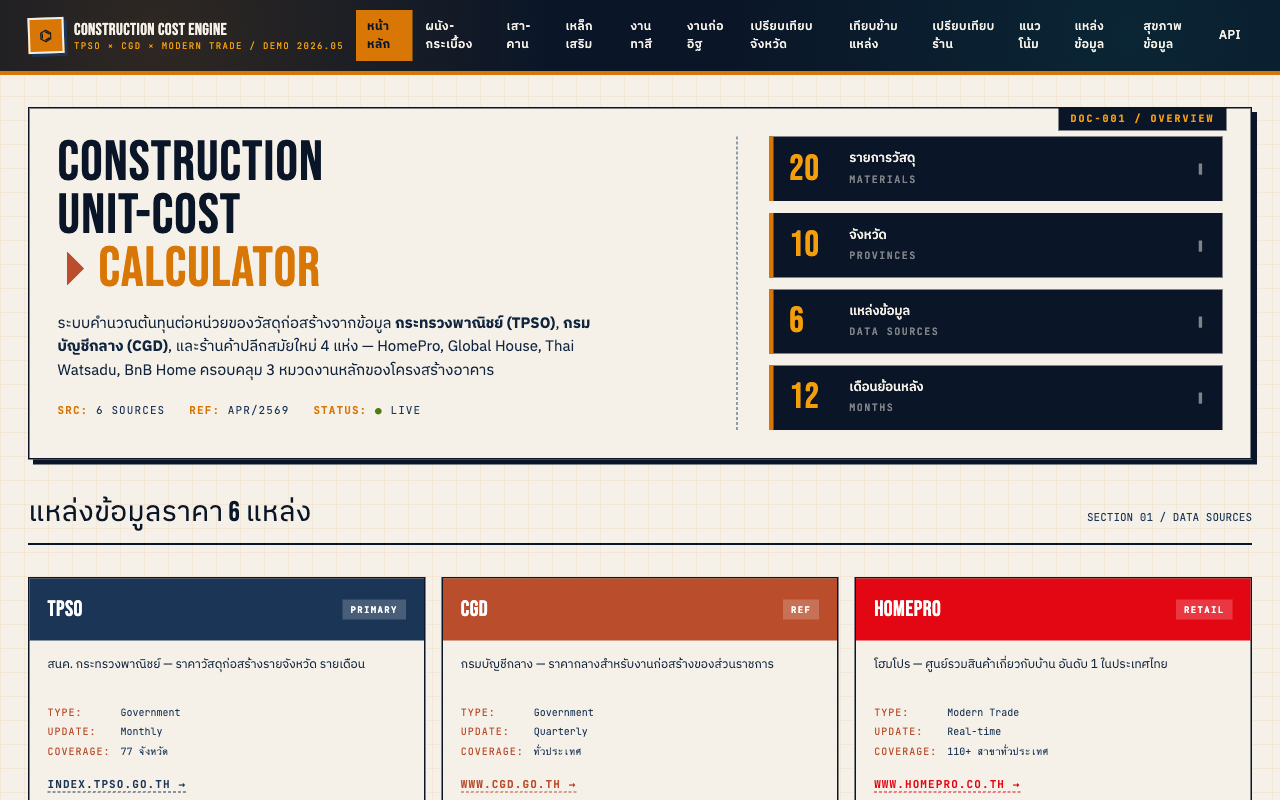
\includegraphics[width=0.95\textwidth]{figures/screen-home.png}
  \caption{หน้าหลัก (\texttt{/}) ของระบบ. แสดงสรุปจำนวนแหล่งข้อมูล รายการวัสดุ พื้นที่ครอบคลุม และทางลัดสู่ฟังก์ชันหลักที่วิศวกรประมาณราคาใช้บ่อยที่สุด.}
  \label{fig:scr-home}
\end{figure}


\section{เปรียบเทียบราคาข้ามแหล่ง (\texttt{/compare-sources})}
% figures/screenshot-compare.tex — production screenshot of /compare-sources
\begin{figure}[H]
  \centering
  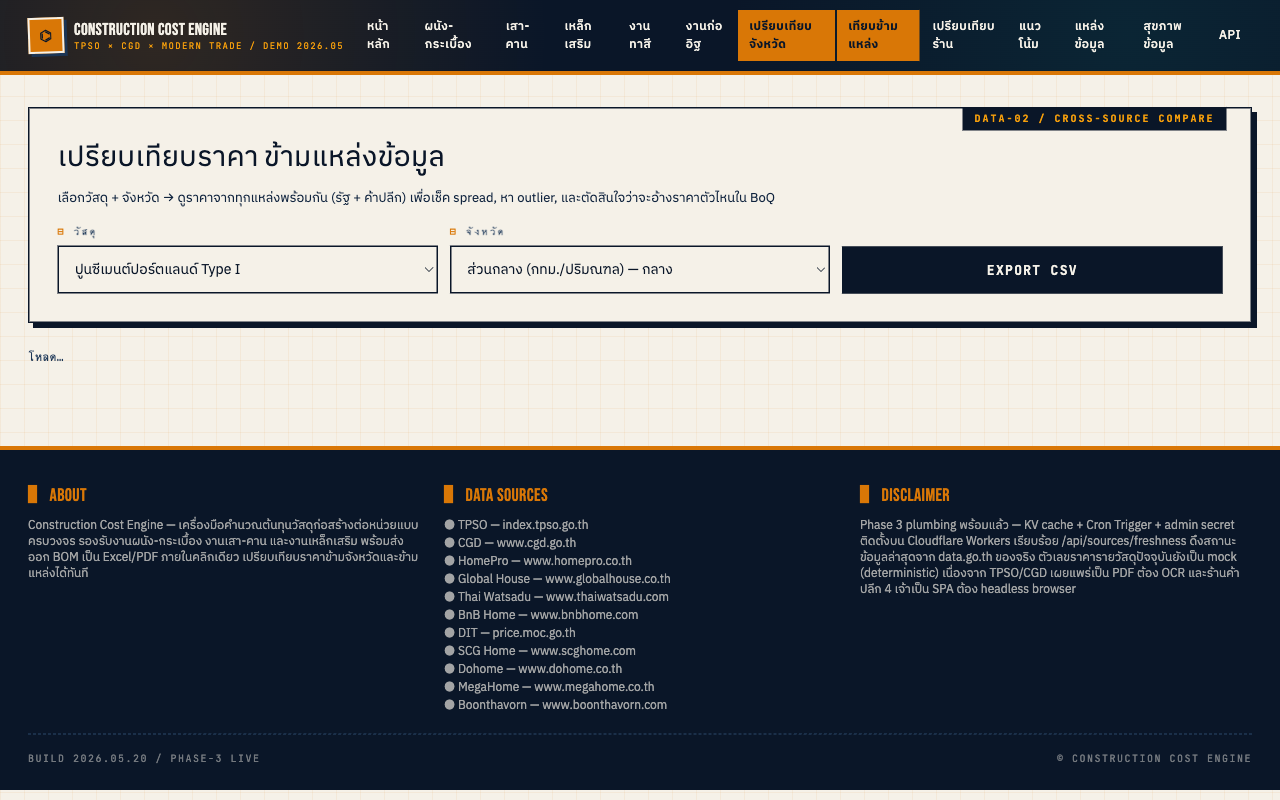
\includegraphics[width=0.95\textwidth]{figures/screen-compare.png}
  \caption{หน้าเปรียบเทียบราคา (\texttt{/compare-sources}). ตารางแสดงราคาเทียบจาก 11 แหล่งข้อมูล ทั้งภาครัฐและภาคค้าปลีกสมัยใหม่ พร้อมเวลา freshness และ flag ราคาที่อาจเป็น outlier.}
  \label{fig:scr-compare}
\end{figure}


\section{แนวโน้มราคา (\texttt{/trend})}
% figures/screenshot-trend.tex — production screenshot of /trend
\begin{figure}[H]
  \centering
  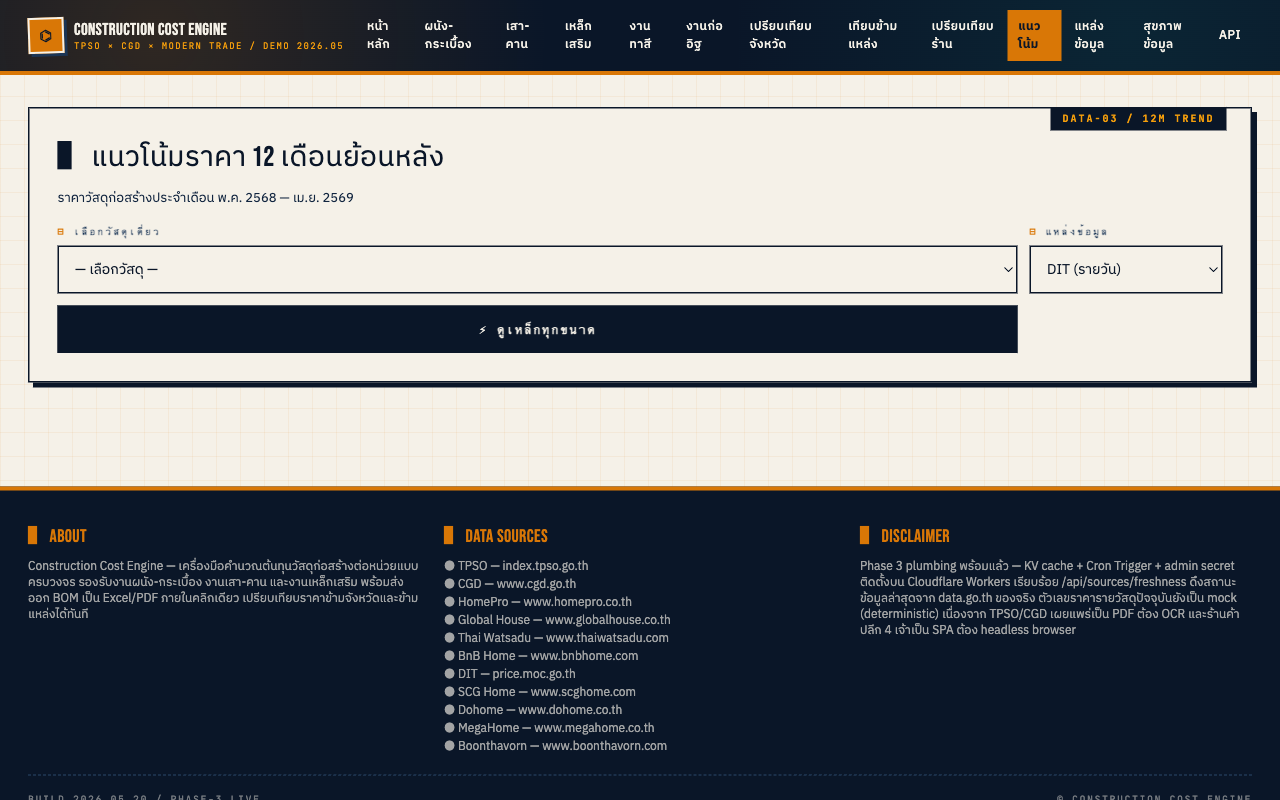
\includegraphics[width=0.95\textwidth]{figures/screen-trend.png}
  \caption{หน้าแนวโน้มราคา (\texttt{/trend}) แสดงดัชนี TPSO CMI 9 เดือน พร้อมเส้นแนวโน้มเชิงเส้น ($R^{2} = 0.989$). ตัวเลขสรุปด้านขวาเป็นข้อมูลที่วิศวกรประมาณราคาใช้เผื่อในงบประมาณโครงการระยะยาว.}
  \label{fig:scr-trend}
\end{figure}


\section{เครื่องคิดเลข BoQ (\texttt{/wall-tile}, \texttt{/paint}, \ldots)}
% figures/screenshot-walltile.tex — UI mockup of /wall-tile (BOQ calculator)
\begin{figure}[H]
  \centering
  \begin{tikzpicture}[font=\scriptsize]
    \draw[draw=gray!50,fill=gray!3,rounded corners=4pt] (0,0) rectangle (12,8);
    \draw[fill=blue!25,draw=blue!50] (0,7.3) rectangle (12,8);
    \node[anchor=west,font=\bfseries] at (0.3,7.65) {คำนวณ BOQ — งานบุกระเบื้องผนัง};

    % Input panel (left)
    \draw[fill=white,draw=gray!50,rounded corners=2pt] (0.3,1.0) rectangle (5.7,7.0);
    \node[anchor=west,font=\bfseries] at (0.5,6.7) {ข้อมูลงาน};
    \node[anchor=west] at (0.5,6.2) {พื้นที่ผนัง (ตร.ม.):};
    \draw[fill=gray!10] (3.0,6.0) rectangle (5.5,6.4); \node[font=\bfseries] at (4.25,6.2) {50};
    \node[anchor=west] at (0.5,5.6) {ขนาดกระเบื้อง:};
    \draw[fill=gray!10] (3.0,5.4) rectangle (5.5,5.8); \node at (4.25,5.6) {30 $\times$ 30 ซม.};
    \node[anchor=west] at (0.5,5.0) {เกรด:};
    \draw[fill=gray!10] (3.0,4.8) rectangle (5.5,5.2); \node at (4.25,5.0) {เกรด A};
    \node[anchor=west] at (0.5,4.4) {ปูนกาว:};
    \draw[fill=gray!10] (3.0,4.2) rectangle (5.5,4.6); \node at (4.25,4.4) {กาวซีเมนต์ 20 กก.};
    \node[anchor=west] at (0.5,3.8) {ภูมิภาค:};
    \draw[fill=gray!10] (3.0,3.6) rectangle (5.5,4.0); \node at (4.25,3.8) {ภาคตะวันออกเฉียงเหนือ};
    \node[anchor=west] at (0.5,3.2) {แหล่งราคา:};
    \draw[fill=gray!10] (3.0,3.0) rectangle (5.5,3.4); \node at (4.25,3.2) {Modern Trade เฉลี่ย};

    \draw[fill=blue!60,draw=blue!80,rounded corners=2pt] (1.0,1.5) rectangle (5.0,2.2);
    \node[white,font=\bfseries] at (3.0,1.85) {คำนวณต้นทุน};

    % Result panel (right)
    \draw[fill=green!5,draw=green!50,rounded corners=2pt] (6.1,1.0) rectangle (11.7,7.0);
    \node[anchor=west,font=\bfseries] at (6.3,6.7) {Bill of Materials};
    \draw[draw=gray!40] (6.3,6.5) -- (11.5,6.5);
    \foreach \i/\m/\q/\u/\p in {
      0/{กระเบื้อง 30$\times$30}/55/แผ่น/{8\,250},
      1/ปูนกาว 20 กก./4/ถุง/{1\,720},
      2/ยาแนว/2/ถุง/{420},
      3/spacer 3 มม./1/ถุง/{180}
    } {
      \node[anchor=west] at (6.3,6.0 - \i*0.45) {\m};
      \node[anchor=east] at (8.5,6.0 - \i*0.45) {\q};
      \node[anchor=west,gray!70] at (8.6,6.0 - \i*0.45) {\u};
      \node[anchor=east,font=\bfseries] at (11.5,6.0 - \i*0.45) {\p};
    }
    \draw[draw=gray!40] (6.3,3.9) -- (11.5,3.9);
    \node[anchor=west,font=\bfseries] at (6.3,3.6) {รวมต้นทุนวัสดุ};
    \node[anchor=east,font=\bfseries] at (11.5,3.6) {10\,570 บาท};
    \node[anchor=west,gray!70,font=\scriptsize] at (6.3,3.2) {ราคาเฉลี่ย/ตร.ม.};
    \node[anchor=east,font=\bfseries,gray!70] at (11.5,3.2) {211 บาท};

    % Export buttons
    \draw[fill=gray!20,draw=gray!50,rounded corners=2pt] (6.3,1.4) rectangle (8.3,2.0);
    \node[font=\scriptsize\bfseries] at (7.3,1.7) {Export Excel};
    \draw[fill=gray!20,draw=gray!50,rounded corners=2pt] (8.6,1.4) rectangle (10.6,2.0);
    \node[font=\scriptsize\bfseries] at (9.6,1.7) {Export PDF};
  \end{tikzpicture}
  \caption{หน้าคำนวณ BOQ งานบุกระเบื้องผนัง (\texttt{/wall-tile}). ผู้ใช้ป้อนพื้นที่งาน ขนาดกระเบื้อง และเลือกแหล่งราคา ระบบจะคำนวณ Bill of Materials ตามหลักเกณฑ์การคำนวณราคากลางของกรมบัญชีกลาง พร้อมรองรับการ export เป็น Excel/PDF เพื่อใช้ในเอกสารโครงการ.}
  \label{fig:scr-walltile}
\end{figure}


\section{สุขภาพแหล่งข้อมูล (\texttt{/health})}
% figures/screenshot-health.tex — UI mockup of /health (system status)
\begin{figure}[H]
  \centering
  \begin{tikzpicture}[font=\scriptsize]
    \draw[draw=gray!50,fill=gray!3,rounded corners=4pt] (0,0) rectangle (12,7.5);
    \draw[fill=blue!25,draw=blue!50] (0,6.8) rectangle (12,7.5);
    \node[anchor=west,font=\bfseries] at (0.3,7.15) {สถานะระบบ — System Health};

    % Overall status badge
    \draw[fill=green!30,draw=green!60,rounded corners=4pt] (0.3,5.9) rectangle (3.5,6.5);
    \node[font=\bfseries] at (1.9,6.2) {\textcolor{green!50!black}{$\bullet$ ปกติ (Healthy)}};

    % Stats summary row
    \foreach \x/\v/\l in {0.3/9/{แหล่ง online}, 3.2/2/{แหล่ง degraded}, 6.1/0/{แหล่ง offline}, 9.0/4.7\%/{outlier rate}} {
      \draw[fill=white,draw=gray!40,rounded corners=2pt] (\x,4.9) rectangle (\x+2.7,5.6);
      \node[font=\bfseries] at (\x+1.35,5.35) {\v};
      \node[font=\scriptsize,gray!70] at (\x+1.35,5.05) {\l};
    }

    % Per-source table
    \node[anchor=west,font=\bfseries] at (0.3,4.5) {รายแหล่ง (cron job last run)};
    \draw[fill=gray!15] (0.3,3.95) rectangle (11.7,4.3);
    \node[anchor=west,font=\bfseries] at (0.5,4.13) {Source};
    \node[anchor=west,font=\bfseries] at (4.0,4.13) {Status};
    \node[anchor=west,font=\bfseries] at (6.5,4.13) {Last update};
    \node[anchor=west,font=\bfseries] at (9.5,4.13) {Records};

    \foreach \i/\src/\st/\time/\rec/\c in {
      0/TPSO/{$\bullet$ ok}/{2 ชม.}/{216}/green,
      1/CGD/{$\bullet$ ok}/{6 ชม.}/{ 24}/green,
      2/DIT/{$\bullet$ ok}/{24 ชม.}/{ 18}/green,
      3/HomePro/{$\bullet$ ok}/{1 ชม.}/{120}/green,
      4/MegaHome/{$\bullet$ ok}/{1 ชม.}/{ 96}/green,
      5/บุญถาวร/{$\bullet$ ok}/{2 ชม.}/{ 48}/green,
      6/ไทวัสดุ/{$\bullet$ ok}/{2 ชม.}/{ 72}/green,
      7/โกลบอลเฮ้าส์/{$\bullet$ degraded}/{14 ชม.}/{ 18}/orange!50!black,
      8/ดูโฮม/{$\bullet$ ok}/{3 ชม.}/{ 24}/green,
      9/เอสซีจีโฮม/{$\bullet$ ok}/{1 ชม.}/{ 12}/green,
      10/บีเอ็นบีโฮม/{$\bullet$ degraded}/{18 ชม.}/{  6}/orange!50!black
    } {
      \node[anchor=west] at (0.5,3.7 - \i*0.30) {\src};
      \node[anchor=west,\c] at (4.0,3.7 - \i*0.30) {\st};
      \node[anchor=west] at (6.5,3.7 - \i*0.30) {\time};
      \node[anchor=west,font=\ttfamily] at (9.5,3.7 - \i*0.30) {\rec};
    }
  \end{tikzpicture}
  \caption{หน้า \texttt{/health} แสดงสถานะระบบและความสดของข้อมูลแต่ละแหล่ง. คอลัมน์ ``Last update'' เป็นข้อมูลที่วิศวกรประมาณราคาใช้ตัดสินว่าราคาในระบบปัจจุบันเชื่อถือได้สำหรับโครงการเร่งด่วนหรือไม่ — แหล่งที่ \texttt{degraded} จะแสดงราคาล่าสุดที่ดึงสำเร็จพร้อม timestamp.}
  \label{fig:scr-health}
\end{figure}


% appendix/B-code-listings.tex
\chapter{ตัวอย่างโค้ดสำคัญของระบบ}
\label{app:code}

\section{Outlier Detection (Z-score)}
\begin{lstlisting}[language=TypeScript,caption={src/lib/stats/outlier.ts}]
export function detectOutliers(values: number[], threshold = 2.0) {
  if (values.length < 3) return values.map(v => ({value: v, zScore: 0, isOutlier: false}));
  const mean = values.reduce((s, v) => s + v, 0) / values.length;
  const std = Math.sqrt(values.reduce((s, v) => s + (v - mean) ** 2, 0) / values.length);
  if (std === 0) return values.map(v => ({value: v, zScore: 0, isOutlier: false}));
  return values.map(v => {
    const z = Math.abs((v - mean) / std);
    return { value: v, zScore: +z.toFixed(2), isOutlier: z > threshold };
  });
}
\end{lstlisting}

\section{Linear Trend Y = a + bX}
\begin{lstlisting}[language=TypeScript,caption={src/lib/stats/linearTrend.ts}]
export function linearTrend(values: number[]) {
  const n = values.length;
  if (n < 2) return null;
  const xs = values.map((_, i) => i);
  const meanX = (n - 1) / 2;
  const meanY = values.reduce((s, v) => s + v, 0) / n;
  let ssXY = 0, ssXX = 0, ssYY = 0;
  for (let i = 0; i < n; i++) {
    ssXY += (xs[i] - meanX) * (values[i] - meanY);
    ssXX += (xs[i] - meanX) ** 2;
    ssYY += (values[i] - meanY) ** 2;
  }
  const b = ssXX === 0 ? 0 : ssXY / ssXX;
  const a = meanY - b * meanX;
  const r2 = ssYY === 0 ? 1 : (ssXY ** 2) / (ssXX * ssYY);
  return { a, b, r2, forecast: (x: number) => a + b * x };
}
\end{lstlisting}

\section{BoQ Calculator (Wall Tile)}
\begin{lstlisting}[language=TypeScript,caption={src/lib/calculators.ts (excerpt)}]
export function calcWallTile(source, province, area, tileId, prices) {
  const items = [];
  items.push(buildItem(prices, source, tileId, area * MATERIALS[tileId].cons));
  items.push(buildItem(prices, source, "ADHESIVE_001", area * 0.25));
  items.push(buildItem(prices, source, "GROUT_001",    area * 0.30));
  items.push(buildItem(prices, source, "PVC_TRIM_001", area * 0.40));
  items.push(buildItem(prices, source, "WATER_MIX_001",area * 0.005));
  const total = items.reduce((s, i) => s + i.total, 0);
  return { workName: "งานผนัง-กระเบื้อง", source, province, items,
           total, unitCost: total / area, unitLabel: "บาท / ตร.ม." };
}
\end{lstlisting}

\section{Cross-source comparison API (\texttt{/api/compare/[material]})}
\begin{lstlisting}[language=TypeScript,caption={Endpoint สำหรับ fan-out 11 แหล่ง}]
export async function GET(req, { params }) {
  const { material } = await params;
  const province = +new URL(req.url).searchParams.get("province") || 10;
  const sources = await Promise.all(
    SOURCE_KEYS.map(async k => {
      const r = await getLivePrice(k, material, province);
      return { source: k, price: r.price, fetchedAt: r.fetchedAt };
    })
  );
  const live = sources.filter(s => s.price != null).map(s => s.price);
  const summary = {
    min: Math.min(...live), max: Math.max(...live),
    median: median(live), avg: live.reduce((s, x) => s + x, 0) / live.length,
    spreadPct: ((Math.max(...live) - Math.min(...live)) / Math.min(...live)) * 100,
  };
  return NextResponse.json({ material, province, sources, summary });
}
\end{lstlisting}

\section{AI Agent Research Endpoint (\texttt{/api/admin/ai-agent})}
\begin{lstlisting}[language=TypeScript,caption={src/app/api/admin/ai-agent/route.ts (excerpt)}]
// Endpoint รับราคาจาก AI Agent (LLM-based) และเขียนลงทั้ง live + history KV
export async function POST(req: Request) {
  const { kv, token } = await getEnv();
  const reqToken = req.headers.get("x-admin-token");
  if (token && reqToken !== token) return NextResponse.json({ error: "unauthorized" }, { status: 401 });

  const body: { source: string; province: number; prices: Record<string, number>; date?: string }
    = await req.json();

  const today = body.date ?? new Date().toISOString().slice(0, 10);
  const written: string[] = [];

  for (const [materialId, raw] of Object.entries(body.prices)) {
    if (!MATERIALS[materialId]) continue;
    const price = Number(raw);
    if (!Number.isFinite(price) || price <= 0) continue;

    // Write live price (same key as auto-scrapers)
    const priceKey = `${body.source}:${materialId}:${body.province}`;
    await kv.put(priceKey, JSON.stringify({ price, fetchedAt: Date.now() }), {
      expirationTtl: DEFAULT_TTL[body.source] ?? 86400,
    });

    // Append to history time-series
    const histKey = `history:${body.source}:${materialId}:${body.province}`;
    const existing = (await kv.get<HistoryEntry[]>(histKey, "json")) ?? [];
    if (!existing.some(e => e.date === today)) {
      existing.push({ date: today, price });
      await kv.put(histKey, JSON.stringify(existing));
    }
    written.push(materialId);
  }
  return NextResponse.json({ ok: true, source: body.source, written: written.length, writtenIds: written });
}
\end{lstlisting}

\section{Boonthavorn GraphQL Scraper}
\begin{lstlisting}[language=TypeScript,caption={src/lib/scrapers/boonthavorn.ts}]
// Boonthavorn ใช้ Magento GraphQL API — ไม่ต้องใช้ ScrapingBee
export const boonthavornProvider: PriceProvider = {
  key: "boonthavorn",
  ttlSec: 60 * 60 * 24 * 30,
  async fetch(materialId: string): Promise<number | null> {
    const q = searchTermFor(materialId);
    const r = await fetch("https://www.boonthavorn.com/graphql", {
      method: "POST",
      headers: { "content-type": "application/json" },
      body: JSON.stringify({
        query: `{ products(search: "${q}" pageSize: 10) {
          items { name price_range { minimum_price { regular_price { value } } } }
        } }`,
      }),
      signal: AbortSignal.timeout(15_000),
    });
    if (!r.ok) return null;
    const data = await r.json();
    return pickBestPrice(data.data.products.items, materialId);
  },
};
\end{lstlisting}

% appendix/C-raw-data.tex
\chapter{ข้อมูลดิบที่ใช้ในระบบ}
\label{app:rawdata}

ข้อมูลในภาคผนวกนี้ดึงจากระบบจริงผ่าน endpoint
\texttt{/api/prices/\{source\}/\{material\}?province=10}
(snapshot 25 พ.ค.\ 2569, กรุงเทพมหานคร). ระบบมีข้อมูลครบ
297/297 cells (11 แหล่ง $\times$ 27 วัสดุ, coverage 100\%).

\section{ราคาวัสดุก่อสร้างจาก 5 แหล่งหลัก (กรุงเทพฯ, 25 พ.ค.\ 2569)}

\begingroup\footnotesize
\begin{longtable}{llrrrrr}
\caption{ราคาวัสดุก่อสร้างเปรียบเทียบ 5 แหล่ง (บาท/หน่วย, province 10)}\\
\toprule
\textbf{Material ID} & \textbf{หน่วย} & \textbf{CGD} & \textbf{DIT} & \textbf{HomePro} & \textbf{Boonthavorn} & \textbf{MegaHome} \\
\midrule
\endhead
CEMENT\_001 & ถุง 50 กก. & 175 & 195 & 185 & 215 & 193 \\
SAND\_001 & ลบ.ม. & 480 & 510 & 82* & 540 & 2{,}690* \\
ROCK\_001 & ลบ.ม. & 650 & 680 & 720 & 720 & 715 \\
TILE\_001 & ตร.ม. & 220 & 245 & 249 & 289 & 242 \\
TILE\_002 & ตร.ม. & 195 & 205 & 280 & 500 & 619 \\
ADHESIVE\_001 & ถุง 20 กก. & 180 & 189 & 193 & 499 & 172 \\
GROUT\_001 & ถุง 1 กก. & 65 & 68 & 83 & 63 & 93 \\
PVC\_TRIM\_001 & เส้น 2.5 ม. & 150 & 165 & 132 & 176 & 143 \\
REBAR\_RB6 & ตัน & 25{,}500 & 26{,}775 & 42{,}351 & 42{,}351 & 42{,}351 \\
REBAR\_RB9 & ตัน & 25{,}000 & 26{,}250 & 41{,}250 & 41{,}250 & 41{,}250 \\
REBAR\_DB10 & ตัน & 24{,}800 & 26{,}040 & 39{,}266 & 39{,}266 & 39{,}266 \\
REBAR\_DB12 & ตัน & 24{,}200 & 24{,}800 & 40{,}436 & 8{,}220* & 26{,}620 \\
REBAR\_DB16 & ตัน & 23{,}900 & 25{,}095 & 40{,}042 & 40{,}042 & 40{,}042 \\
REBAR\_DB20 & ตัน & 23{,}700 & 24{,}885 & 33{,}250 & 33{,}250 & 33{,}250 \\
REBAR\_DB25 & ตัน & 23{,}500 & 24{,}675 & 40{,}043 & 40{,}043 & 40{,}043 \\
WIRE\_001 & กก. & 38 & 40 & 85 & 85 & 57 \\
FORM\_WOOD\_001 & แผ่น 1.2x2.4 ม. & 520 & 546 & 650 & 7{,}590 & 680 \\
NAIL\_001 & กก. & 42 & 44 & 105 & 165 & 109 \\
PAINT\_INT\_001 & แกลลอน & 1{,}250 & 1{,}290 & 625 & 1{,}350 & 1{,}375 \\
PAINT\_EXT\_001 & แกลลอน & 1{,}590 & 1{,}650 & 795 & 1{,}750 & 1{,}749 \\
PRIMER\_001 & แกลลอน & 820 & 861 & 1{,}500 & 890 & 902 \\
BRICK\_001 & 100 ก้อน & 180 & 190 & 200 & 210 & 198 \\
BRICK\_002 & ก้อน & 2{,}200 & 2{,}310 & 43 & 3{,}200 & 45 \\
CONCRETE\_240 & ลบ.ม. & 2{,}800 & 2{,}900 & 2{,}900 & 3{,}200 & 3{,}080 \\
CONCRETE\_280 & ลบ.ม. & 3{,}100 & 3{,}255 & 3{,}255 & 3{,}500 & 3{,}410 \\
WATER\_MIX\_001 & ลบ.ม. & 16 & 16 & 16 & 16 & 16 \\
WATER\_MIX\_002 & ลบ.ม. & 16 & 16 & 16 & 16 & 16 \\
\bottomrule
\multicolumn{7}{l}{\small * หมายเหตุ: ราคาที่มี * อาจมีความแตกต่างของหน่วยบรรจุภัณฑ์ (เช่น per bag vs per m\textsuperscript{3})} \\
\end{longtable}
\endgroup

\section{TPSO ราคาปูนซีเมนต์ Type I กรุงเทพมหานคร (10 เดือน)}

\begin{table}[H]\centering
\caption{ราคาปูนซีเมนต์ Type I (50 กก.) จาก TPSO กรุงเทพมหานคร
(ดึงจาก \texttt{/api/history/tpso/CEMENT\_001}, snapshot 25 พ.ค.\ 2569)}
\label{tab:tpso-history}
\begin{tabularx}{\textwidth}{lrr}
\toprule
\textbf{วันที่} & \textbf{ราคา (บาท/ถุง)} & \textbf{$\Delta$\% MoM} \\
\midrule
ส.ค.\ 2568 & 171.00 & --- \\
ก.ย.\ 2568 & 171.00 & 0.00\% \\
ต.ค.\ 2568 & 172.00 & $+$0.58\% \\
พ.ย.\ 2568 & 173.00 & $+$0.58\% \\
ธ.ค.\ 2568 & 173.00 & 0.00\% \\
ม.ค.\ 2569 & 174.00 & $+$0.58\% \\
ก.พ.\ 2569 & 174.00 & 0.00\% \\
มี.ค.\ 2569 & 175.00 & $+$0.57\% \\
เม.ย.\ 2569 & 175.00 & 0.00\% \\
21 พ.ค.\ 2569 & 179.45 & $+$2.54\% \\
25 พ.ค.\ 2569 & 179.45 & 0.00\% \\
\midrule
\textbf{รวม} & \multicolumn{2}{r}{\textbf{$+$8.45 บาท ($+$4.9\%) ใน 10 เดือน}} \\
\bottomrule
\end{tabularx}
\end{table}

\section{TPSO CMI ดัชนีราคาวัสดุก่อสร้าง (ล่าสุด)}

\begin{table}[H]\centering
\caption{ดัชนีราคาวัสดุก่อสร้างของกระทรวงพาณิชย์ (TPSO CMI, base 2563=100,
ดึงจาก \texttt{/api/sources/tpso/cmi})}
\label{tab:cmi-latest}
\begin{tabularx}{\textwidth}{lX}
\toprule
\textbf{ตัวชี้วัด} & \textbf{ค่า} \\
\midrule
Index ล่าสุด & 112.8 (มีนาคม 2568) \\
Baseline & 110.0 \\
CMI Ratio & 1.0255 \\
YoY \% & $+$0.5\% \\
MoM \% & $+$0.6\% \\
\bottomrule
\end{tabularx}
\end{table}

\section{แหล่งอ้างอิงข้อมูล}

\begin{itemize}
  \item \url{https://construction-cost-engine.steep-tooth-c420.workers.dev/api/sources/health}
        --- สถานะ coverage ของระบบ (297/297 cells, 100\%)
  \item \url{https://www.tpso.go.th/} --- TPSO CMI bulletin
  \item \url{https://www.cgd.go.th/} --- กรมบัญชีกลาง ราคามาตรฐาน
  \item \url{https://www.homepro.co.th/service/search/suggest.jsp} --- HomePro JSON API
  \item \url{https://www.megahome.co.th/service/search/suggest.jsp} --- MegaHome JSON API
  \item \url{https://www.boonthavorn.com/graphql} --- Boonthavorn GraphQL API
\end{itemize}


\end{document}
